\documentclass[11pt,letterpaper]{report}

\usepackage[margin=1in]{geometry}
\usepackage{amsmath,amssymb}
\usepackage{graphicx}
\usepackage{booktabs}
\usepackage{siunitx}
\usepackage{hyperref}
\usepackage{xcolor}
\usepackage{caption}
\usepackage{setspace}
\usepackage{enumitem}

\graphicspath{{figures/}}
\hypersetup{
  colorlinks=true,
  linkcolor=blue!50!black,
  urlcolor=blue!50!black,
  citecolor=blue!50!black
}

\sisetup{per-mode=symbol}

\newcommand{\Sd}{S_d}
\newcommand{\fres}{f_{\mathrm{res}}}
\newcommand{\fp}{f_p}
\newcommand{\ImZ}{\operatorname{Im}\{Z\}}
\newcommand{\ReZ}{\operatorname{Re}\{Z\}}


\title{PF-FDTD Sheath study Progress and Analysis Report\\[0.4em]
\large Antenna Impedance in Plasma and Tu (2008) Sheath Validation}
\author{}
\date{}

\begin{document}

\maketitle

\begin{abstract}
This report records the experimental campaign on the Plasma Fluid Finite-Difference Time-Domain (PF-FDTD) solver from the February 2026 dipole-in-plasma baseline through the August 2026 dense continuous-wave (CW) sheath-width sweep. The scientific goal is to reproduce the Tu (2008) result that a vacuum sheath of increasing width \(\Sd\) around a radio-frequency dipole raises the series resonance \(\fres\) toward the free-space value. Early pulse and low-frequency CW campaigns either failed as measurements or showed \(Z\) independent of \(\Sd\). A coupling bug---sheath depletion seeded from the plasma-on mask before antenna geometry existed---placed the density hole at the domain edge rather than next to the wire. After a PEC-seeded fix, feed impedance depends strongly on sheath width. A dense 66-case CW sweep at \(\fp=\SI{2}{\mega\hertz}\) (1.50--2.30~MHz) completed on 18 August 2026: \(\fres(\Sd=0)\approx\SI{1.846}{\mega\hertz}\), but no \(\ImZ\) \(+\) to \(-\) crossing appears for \(\Sd\ge 2\) in that band, so the Tu upward shift was not reproduced with this observable.
\end{abstract}

\tableofcontents

\chapter{Project Goal}
\label{ch:goals}

\section{The solver}

Plasma Fluid Finite-Difference Time-Domain (PF-FDTD) is a three-dimensional electromagnetic solver coupled to multi-species plasma fluid equations. It originated in Jeffrey~D.\ Ward's plasma-frequency-probe work at Utah State University~\cite{ward2006} and has been modernized with a modular \texttt{src/} layout, OpenMP, Python visualization, and scripted experiment drivers.

On a staggered Yee grid the code advances Maxwell's equations
\begin{align}
\nabla \times \mathbf{E} &= -\partial_t\mathbf{B}, \\
\nabla \times \mathbf{B} &= \mu_0\varepsilon_0\,\partial_t\mathbf{E} + \mu_0\mathbf{J},
\end{align}
with plasma current \(\mathbf{J}=\sum_s q_s n_s\mathbf{u}_s\) from continuity and momentum updates for each species. Antenna geometry and sources are read from \texttt{.str} input files. The feed observables used throughout this report are the voltage \(V(t)\) and current \(I(t)\) written to \texttt{.vc} files; input impedance is
\begin{equation}
Z(f)=\frac{V(f)}{I(f)}.
\end{equation}

\section{Scientific target: Tu (2008)}

The active research goal is to reproduce the sheath-induced resonance shift reported by Tu~\cite{tu2008}. A conducting antenna in plasma develops a vacuum (or strongly depleted) sheath of width \(\Sd\) cells next to the conductor. Inside that layer the ambient density is essentially zero; outside it recovers to the bulk \(N_0\).

Increasing \(\Sd\) reduces dielectric loading near the antenna, so the series resonance \(\fres\)---the frequency where \(\ImZ=0\) with a \(+\) to \(-\) crossing---should move \emph{upward} toward the free-space value.

An equivalent-circuit picture of the same effect is a sheath capacitance in series with the antenna feed:
\begin{equation}
Z_{\mathrm{in}}(f)=Z_{\mathrm{ant}}(f)+\frac{1}{j\omega C_{\mathrm{sh}}},
\qquad
C_{\mathrm{sh}}\sim\frac{\varepsilon_0 A}{\Sd\,\Delta x}.
\end{equation}
In FDTD this is realized as a volumetric vacuum gap on Yee nodes adjacent to the conductor: depleted \(N_0\) implies \(J\approx 0\), so those cells act as vacuum capacitors loading the feed. Tu's lumped \(C_{\mathrm{sh}}\) is the circuit limit of that gap; it is not implemented as a separate circuit element.

\section{Campaign protocol}

The planned observable is \(\fres(\Sd)\) for \(\Sd\in\{0,2,4,6,8,10\}\) cells on a \(70\times 70\times 65\) dipole grid with \(\Delta x=\SI{0.04}{\meter}\). The same geometry appears in every chapter of this report: a \(z\)-directed thin-wire dipole from \((35,35,20)\) to \((35,35,45)\) with a hard \(E_z\) source at \((35,35,33)\).

What changed between phases is the excitation (broadband pulse versus CW sine), the plasma frequency, and---after August 2026---whether the sheath was actually attached to the conductor. Each subsequent chapter records what was tried, what succeeded, and what failed.

\section{How to read this document}

Chapters are chronological. Chapter~\ref{ch:february} is the February 2026 free-space versus plasma baseline on this dipole; it is a prerequisite, not a detour. Chapters~\ref{ch:pulse}--\ref{ch:fpscreen} are pre-fix sheath campaigns. Chapter~\ref{ch:fix} diagnoses the coupling bug. Chapters~\ref{ch:confirm}--\ref{ch:cwtu} are post-fix confirmation and the dense CW Tu sweep completed 18 August 2026.

\chapter{February Baseline: Dipole in Free Space versus Plasma}
\label{ch:february}

\section{What we tried}

After the January 2026 modernization (modular sources, CMake, OpenMP, Python plotting), the first physics question was whether the rebuilt solver could show plasma loading of a dipole at all. That is the prerequisite for later asking whether a vacuum sheath \emph{changes} that loading.

All February runs used the same antenna that later became \texttt{sheath.str}: \(70\times 70\times 65\) cells, \(\Delta x=\SI{0.04}{\meter}\), PEC from \((35,35,20)\) to \((35,35,45)\), feed at \((35,35,33)\), type-5 differentiated Gaussian. The only material difference from the May sheath input is the source parameter (\(\SI{100}{\mega\hertz}\) here versus \(\SI{30}{\kilo\hertz}\) later).

\begin{table}[ht]
\centering
\caption{February 2026 dipole runs under \texttt{results/}.}
\label{tab:feb-runs}
\begin{tabular}{@{}llll@{}}
\toprule
Run & Question & Settings & Outcome \\
\midrule
\texttt{production\_run\_8000} & Does OpenMP plasma run? & \(\fp=\SI{5.3}{\mega\hertz}\), \(f_c=\SI{1.43}{\mega\hertz}\), 8k steps & Yes: \(V/I\) and \(Z(f)\) plots \\
\texttt{freespace\_test} & Free-space dipole & no plasma CLI args, 100k steps & Baseline \(Z(f)\) \\
\texttt{ionoplasma\_test} & Plasma on, same dipole & \(\fp=\SI{0.5}{\mega\hertz}\), \(f_g=\SI{1.1}{\mega\hertz}\), 100k steps & Plasma-loaded \(Z(f)\) \\
\texttt{ionoplasma\_test\_5\_1\_11} & Collision / cyclotron variant & \(\fp=\SI{0.5}{\mega\hertz}\), \(f_c=\SI{0.05}{\mega\hertz}\), 64k steps & Parameter sensitivity \\
\texttt{benchmarks} & Legacy vs new OpenMP & \texttt{dipoleTest}, 10k steps & Timing, not physics \\
\texttt{test\_freespace} / \texttt{test\_plasma} & CLI plasma-flag check & \texttt{verify\_plasma\_flag.bat} & Incomplete (empty logs) \\
\bottomrule
\end{tabular}
\end{table}

\section{What succeeded}

The modernized OpenMP executable ran to completion. Free-space and plasma cases produced distinct voltage/current traces and impedance spectra (Figures~\ref{fig:feb-fs}--\ref{fig:feb-plasma}). The Python \(Z(f)=V(f)/I(f)\) pipeline used in every later chapter starts here. OpenMP scaling was recorded in Figure~\ref{fig:scaling}.

This established that \emph{plasma loading of feed impedance is measurable} on this grid. Without that result, a sheath-width sweep would have had no baseline.

\begin{figure}[ht]
\centering
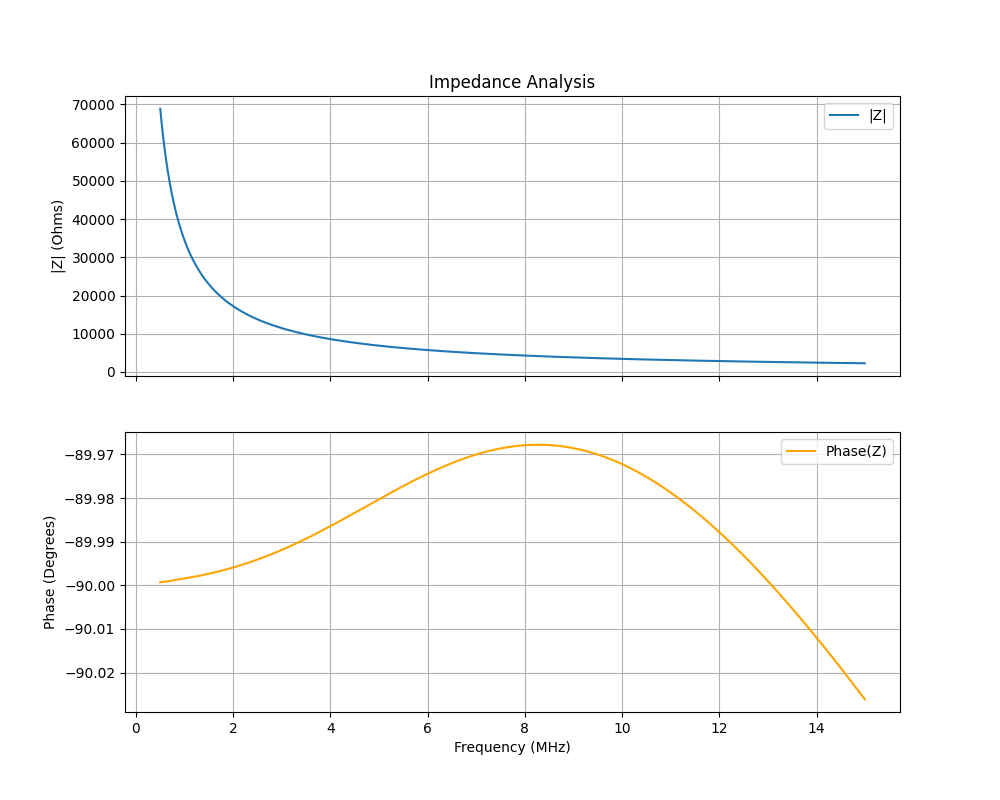
\includegraphics[width=0.85\textwidth]{feb_freespace_impedance.png}
\caption{Free-space dipole impedance from \texttt{results/freespace\_test} (February 2026). Same geometry as all later sheath runs.}
\label{fig:feb-fs}
\end{figure}

\begin{figure}[ht]
\centering
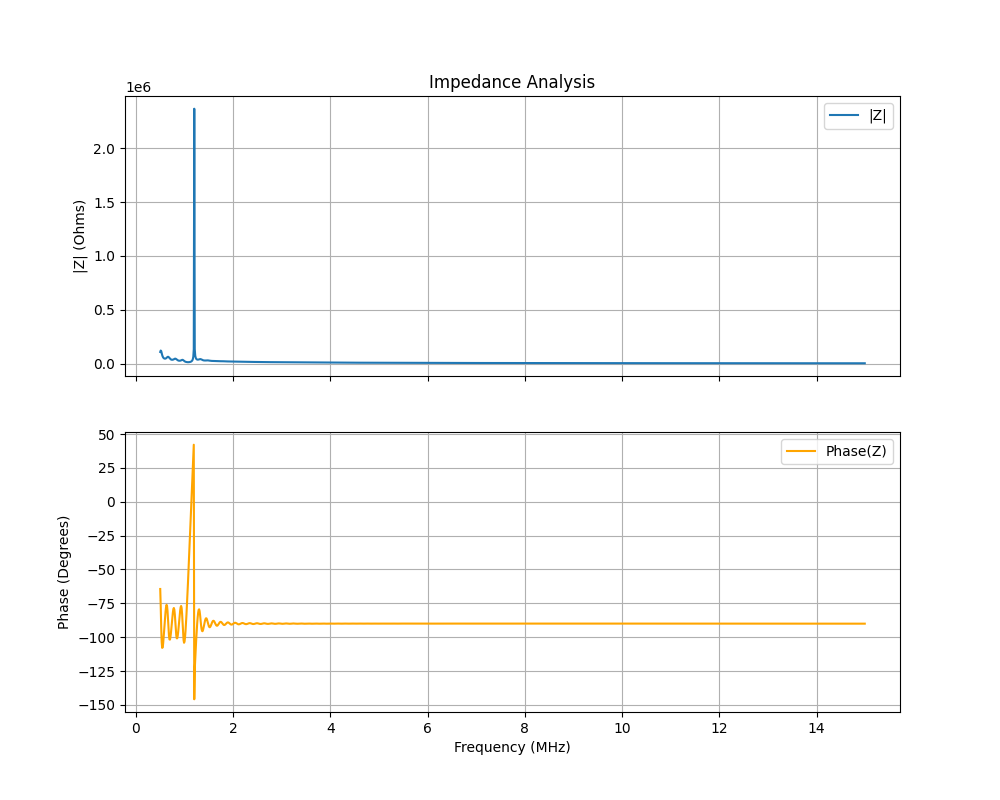
\includegraphics[width=0.85\textwidth]{feb_ionoplasma_impedance.png}
\caption{Plasma-loaded dipole impedance from \texttt{results/ionoplasma\_test} (\(\fp=\SI{0.5}{\mega\hertz}\)). Plasma changes \(Z(f)\) relative to Figure~\ref{fig:feb-fs}.}
\label{fig:feb-plasma}
\end{figure}

\begin{figure}[ht]
\centering
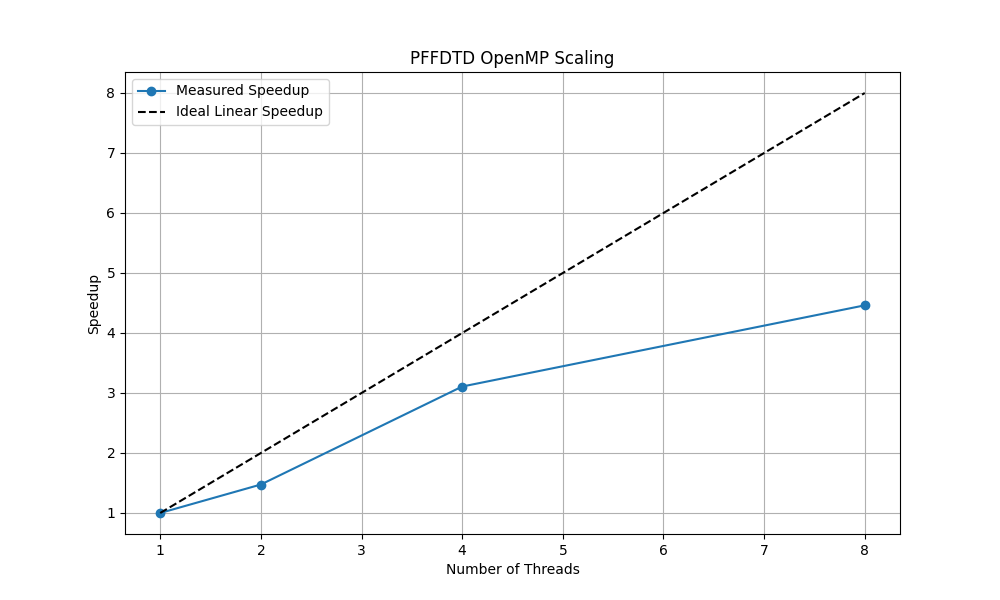
\includegraphics[width=0.75\textwidth]{scaling_results.png}
\caption{OpenMP scaling recorded during the February solver checkout.}
\label{fig:scaling}
\end{figure}

\section{What failed or was left open}

\begin{itemize}[leftmargin=1.5em]
\item There was no sheath parameter \(\Sd\). Density was spatially uniform.
\item Plasma frequencies (\(\SI{5.3}{\mega\hertz}\) or \(\SI{0.5}{\mega\hertz}\)) were Ward-like ionospheric defaults, not yet the Tu-oriented \(\SI{200}{\kilo\hertz}\) then \(\SI{2}{\mega\hertz}\) choices.
\item The \(\SI{100}{\mega\hertz}\) differentiated Gaussian is a broadband pulse. Frequency resolution and spectral artifacts from this class of drive reappear as a measurement failure in Chapter~\ref{ch:pulse}.
\item Several February runs included a cyclotron frequency (background \(\mathbf{B}\)). Later sheath work set \(f_{\mathrm{cyc}}=0\).
\item The CLI plasma-flag stubs (\texttt{test\_freespace}, \texttt{test\_plasma}) did not produce usable logs.
\end{itemize}

The May sheath campaign is the next chapter of this same antenna-in-plasma story: keep the dipole, add a vacuum layer of width \(\Sd\), and look for an upward shift of \(\fres\).

\chapter{Pulse Sheath-Width Sweep}
\label{ch:pulse}

\section{What we tried}

The first sheath campaign (13--16 May 2026) added a step-profile vacuum sheath of width \(\Sd\) cells around the February dipole and drove it with a broadband pulse. The protocol is in \texttt{docs/sheath/SHEATH\_VALIDATION\_IMPLEMENTATION\_PLAN.md}.

\begin{itemize}[leftmargin=1.5em]
\item Input: \texttt{sheath.str} --- source type~5 (differentiated Gaussian) at \(\SI{30}{\kilo\hertz}\).
\item Plasma: \(\fp=\SI{200}{\kilo\hertz}\), \(T=\SI{2000}{\kelvin}\), no background \(\mathbf{B}\).
\item Sheath: \(\Sd=0,2,4,6,8,10\).
\item Analysis: Hanning-window FFT of the full \(V(t)/I(t)\) traces (\texttt{scripts/analyze\_sheath\_results.py}).
\item Data: \texttt{results/sheath\_sweep/}, plus a longer \(\Sd=0\) attempt in \texttt{results/sheath\_long/}.
\end{itemize}

The expected signature was a monotonic increase of \(\fres\) with \(\Sd\).

\section{What failed}

No \(\ImZ=0\) crossing was found below \(\SI{1}{\mega\hertz}\). Fallback \(|Z|\) peaks fell in the multi-gigahertz band (Table~\ref{tab:pulse-peaks}) and are sampling/FFT artifacts, not the kHz/MHz antenna resonance discussed by Tu. A long-trace reanalysis of \texttt{sheath\_long/sd0} with a \(\SI{200}{\kilo\hertz}\) cap still found no zero-crossing (fallback peak \(\SI{46.8}{\kilo\hertz}\)).

\begin{table}[ht]
\centering
\caption{Pulse-FFT ``resonance'' picks from the May \(\Sd\) sweep. All Im\(\{Z\}\) crossings in the analysis band are missing; GHz peaks are not physical.}
\label{tab:pulse-peaks}
\begin{tabular}{@{}rrr@{}}
\toprule
\(\Sd\) (cells) & Im\(\{Z\}\) zero-crossing & Fallback \(|Z|\) peak (Hz) \\
\midrule
0  & --- & \(6.61\times 10^{9}\) \\
2  & --- & \(6.16\times 10^{9}\) \\
4  & --- & \(5.28\times 10^{9}\) \\
6  & --- & \(5.28\times 10^{9}\) \\
8  & --- & \(5.28\times 10^{9}\) \\
10 & --- & \(5.28\times 10^{9}\) \\
\bottomrule
\end{tabular}
\end{table}

\begin{figure}[ht]
\centering
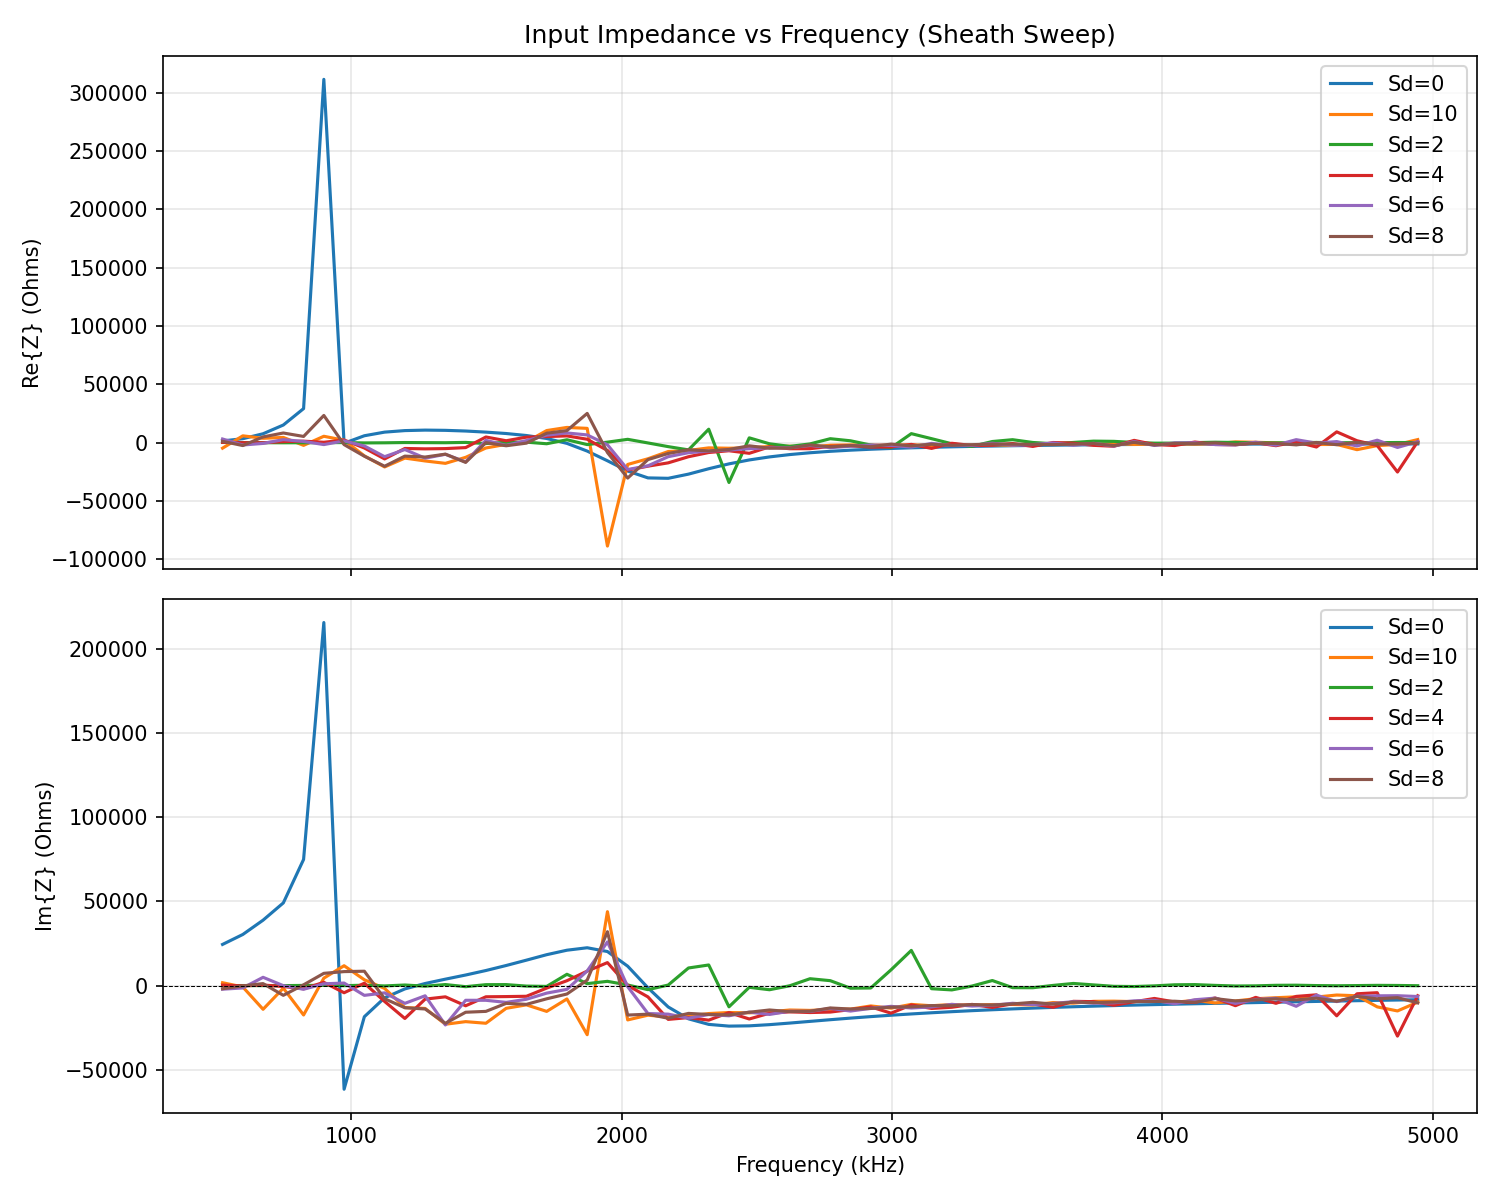
\includegraphics[width=0.9\textwidth]{sheath_impedance.png}
\caption{Broadband pulse FFT impedance versus frequency for \(\Sd=0\ldots 10\). No usable series resonance in the Tu band.}
\label{fig:pulse-z}
\end{figure}

\begin{figure}[ht]
\centering
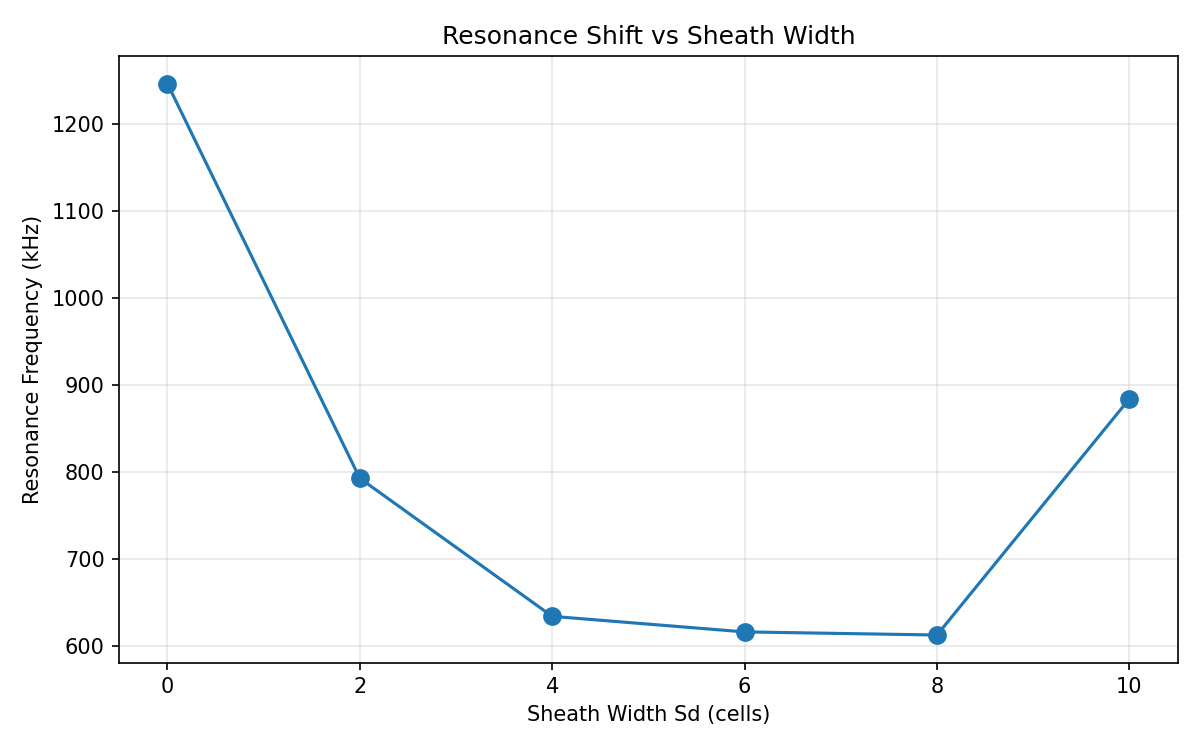
\includegraphics[width=0.85\textwidth]{sheath_resonance_shift.png}
\caption{Apparent resonance versus \(\Sd\) from the pulse analyzer. The GHz-scale picks are FFT artifacts; this campaign cannot test Tu (2008).}
\label{fig:pulse-shift}
\end{figure}

\section{What succeeded, narrowly}

All six \(\Sd\) runs completed and wrote readable \texttt{data.vc} files. The analyzer and sweep scripts became the template for later campaigns. That is an infrastructure success, not a physics result.

\section{Interpretation}

This campaign \emph{cannot test} Tu (2008): the observable \(\fres\) was never resolved. Possible contributors, recorded at the time, were coarse DFT bins at kHz scales, transient-dominated traces, and a drive that did not sit on the resonance. A later finding (Chapter~\ref{ch:fix}) adds a second, independent failure: even a perfect FFT would have seen no \(\Sd\) dependence, because the sheath was not coupled to the feed.

Policy after this phase: do not spend further wall time on long broadband pulse runs until the measurement method is confirmed with narrow-band or CW excitation.

\chapter{Narrow-Band and Two-Dimensional CW below \(\fp\)}
\label{ch:narrow}

\section{What we tried}

Because the pulse FFT did not resolve \(\fres\), the next phase switched to a continuous-wave sine (\texttt{sheath\_sine.str}) and extracted a phasor \(Z=V/I\) from the last half of each trace. Two related campaigns ran from late May through 11 August 2026.

\paragraph{Narrow-band frequency scan.}
\texttt{results/sheath\_narrow\_band/}, driver \texttt{scripts/run\_sheath\_narrow\_band.ps1}. Sixteen frequencies from \(\SI{10}{\kilo\hertz}\) to \(\SI{400}{\kilo\hertz}\). Folder names are \texttt{sd\{\emph{Hz}\}} (for example \texttt{sd20000}): a PowerShell expansion bug treated \(\Sd\) as empty, so these directories are frequencies, not sheath widths. The default \(\Sd\) was 0.

\paragraph{Two-dimensional \(\Sd\times f\) sweep.}
\texttt{results/sheath\_2d\_sweep/}. \(\Sd=0\) at 20--400~kHz; \(\Sd=2,4,6,8,10\) at 100, 150, 200, and 300~kHz. Phasor analysis: \texttt{scripts/analyze\_2d\_sweep.py}.

Both campaigns sit well below the \(\sim\SI{1.8}{\mega\hertz}\) resonance later found near \(\fp=\SI{2}{\mega\hertz}\).

\section{What succeeded}

CW phasor impedance is a stable measurement. Traces reach a usable steady state, and \(\ReZ\) and \(\ImZ\) versus drive frequency are smooth enough to plot (Figures~\ref{fig:narrow}--\ref{fig:twod}). This is the measurement method used for all subsequent screens.

\begin{figure}[ht]
\centering
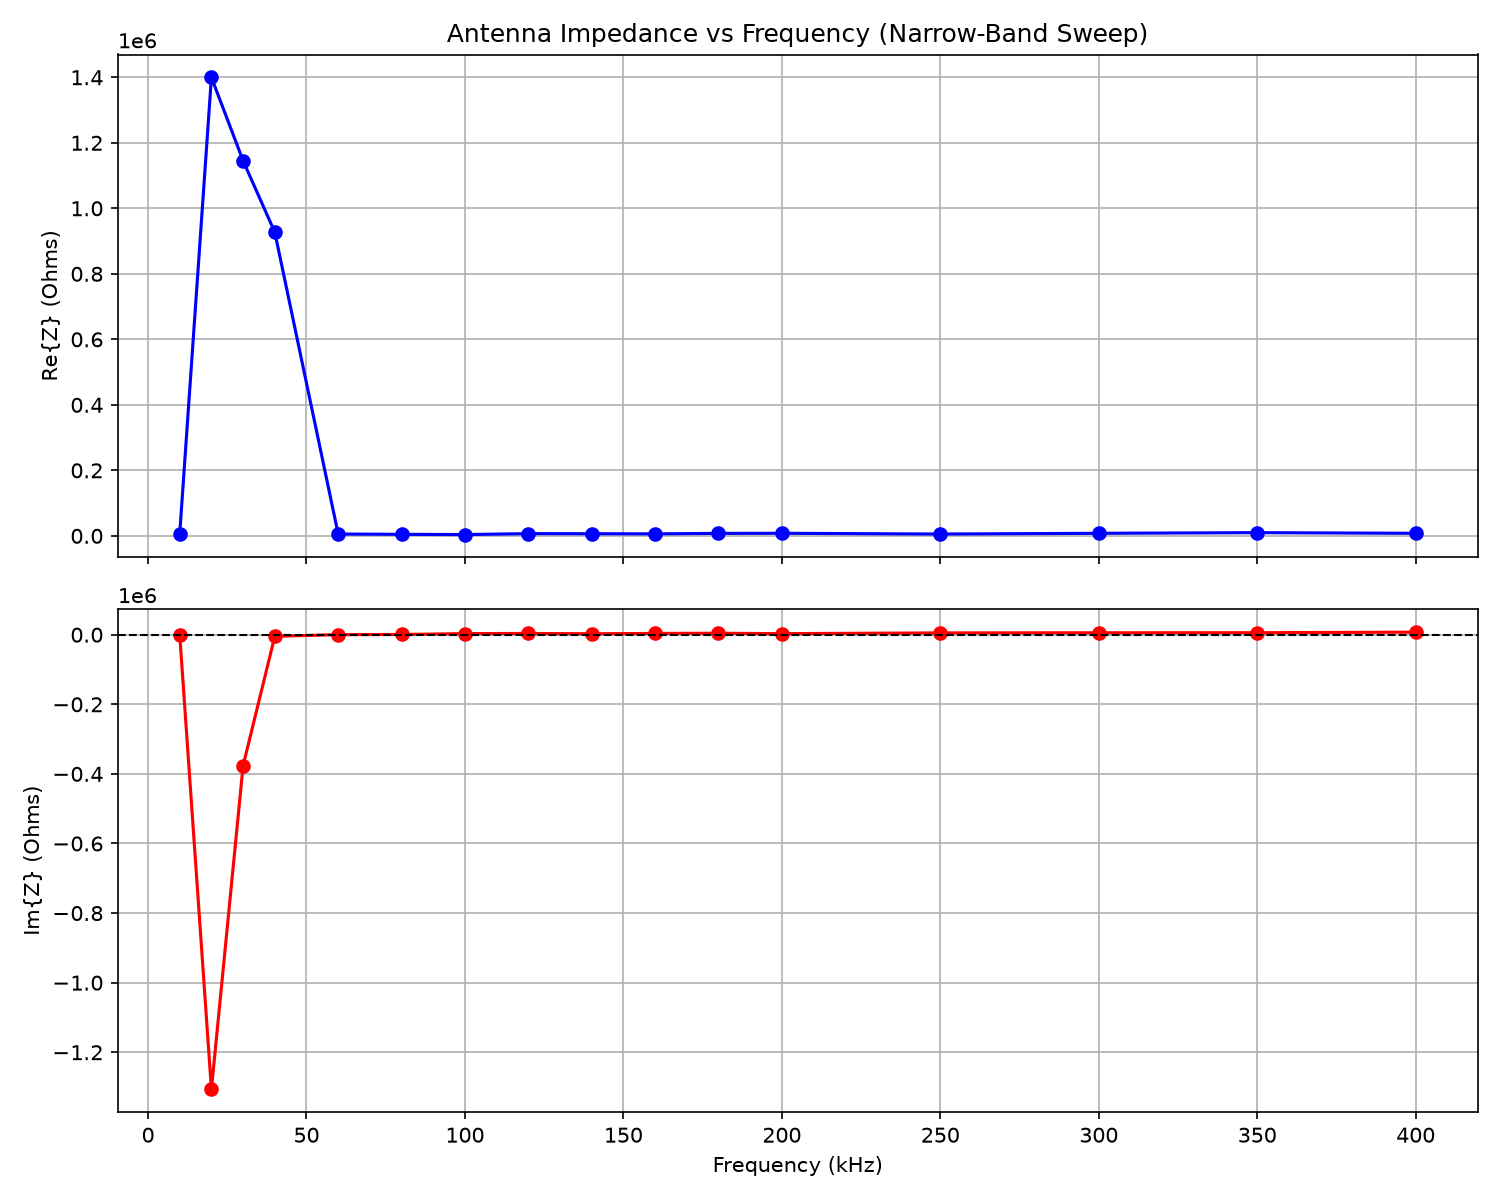
\includegraphics[width=0.9\textwidth]{narrow_band_impedance.png}
\caption{Narrow-band CW impedance, 10--400~kHz. Folders are misnamed \texttt{sd\{Hz\}}; the physical sheath width is the script default \(\Sd=0\).}
\label{fig:narrow}
\end{figure}

\begin{figure}[ht]
\centering
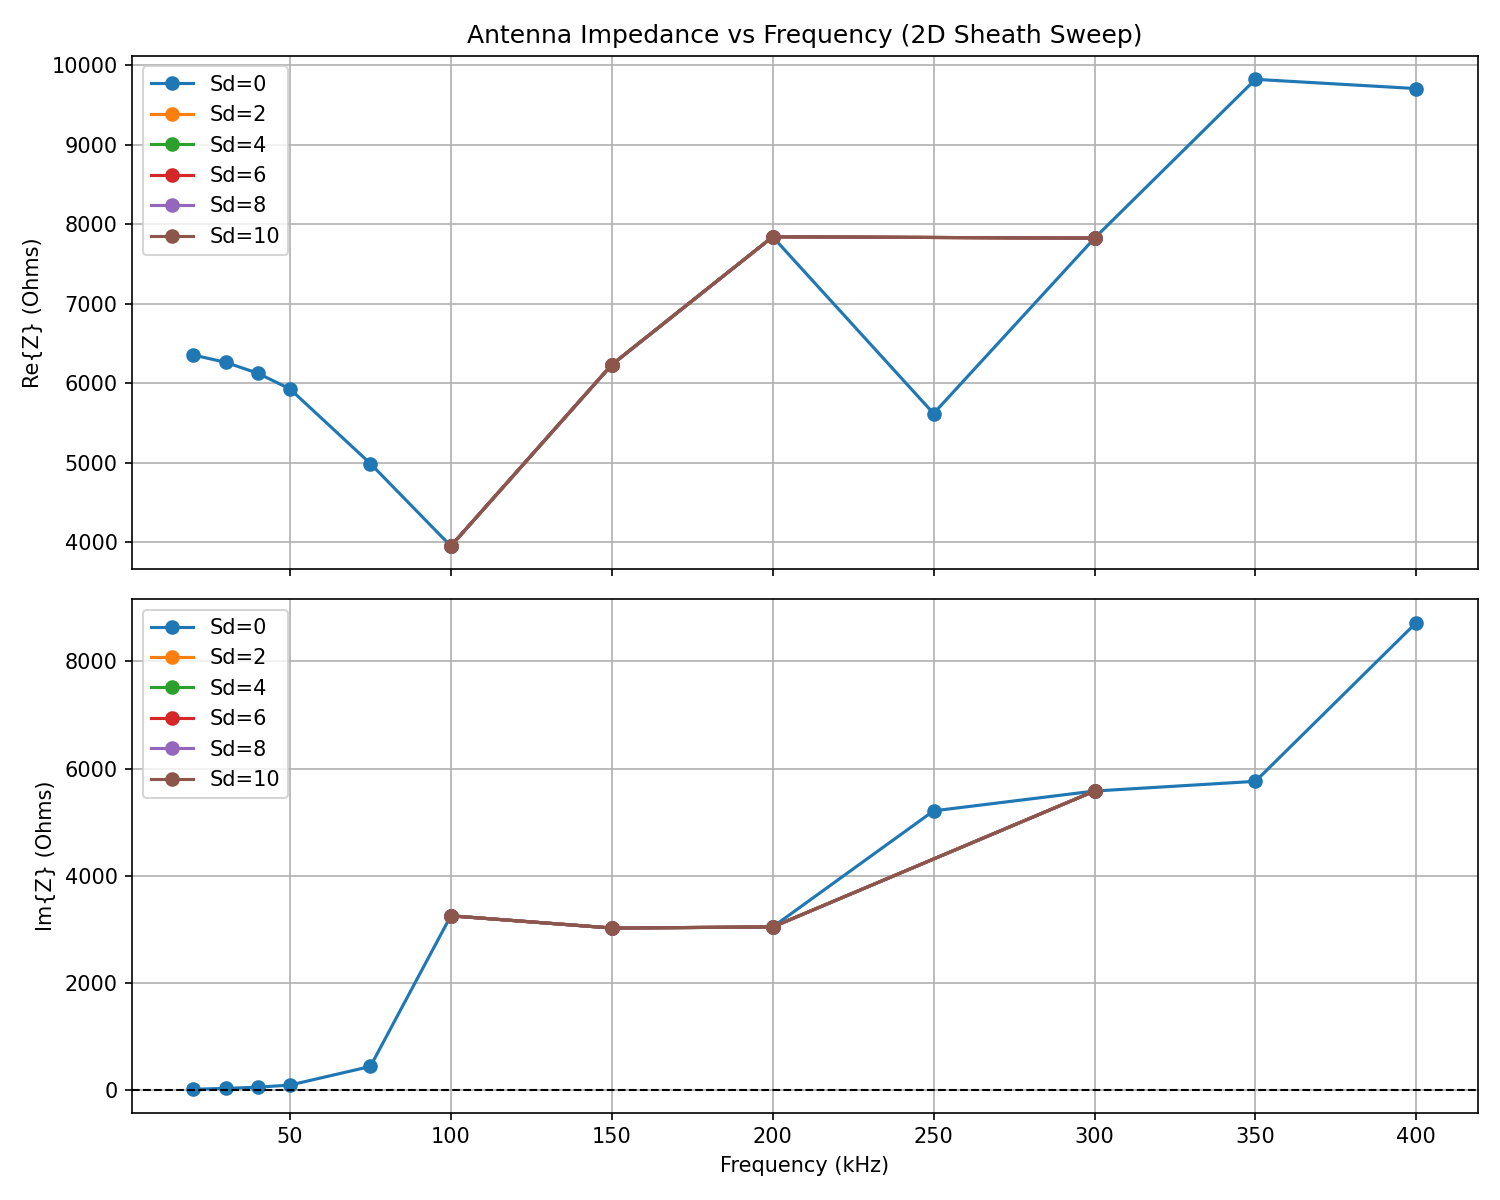
\includegraphics[width=0.9\textwidth]{sheath_2d_sweep_lowf.png}
\caption{Two-dimensional CW sweep at 20--400~kHz. Curves for \(\Sd=2\ldots 10\) overlie one another; sheath width does not enter the feed.}
\label{fig:twod}
\end{figure}

\section{What failed}

The physics test failed, for two stacked reasons.

\begin{enumerate}[leftmargin=1.5em]
\item \textbf{Wrong band.} These frequencies are far below the series feature later located near \(\SI{1.78}{\mega\hertz}\) (Chapter~\ref{ch:fpscreen}). A null result here cannot confirm or refute Tu.
\item \textbf{No \(\Sd\) dependence even where compared.} Tables for \(\Sd=2,4,6,8,10\) at 100--300~kHz are numerically identical to many digits. Example at \(\SI{200}{\kilo\hertz}\): \(\Sd=0\) gives \(\ReZ\approx\SI{7841}{\ohm}\), \(\ImZ\approx\SI{3046}{\ohm}\); \(\Sd=10\) agrees to the reported precision. The sheath never loaded the feed.
\end{enumerate}

The overlapping \(\Sd\) curves in Figure~\ref{fig:twod} are the first clear sign that the volumetric sheath was not attached to the antenna. That conclusion is made definitive by the \(\fp\)-screen in the next chapter, which repeats the comparison \emph{on} the resonance.

\chapter{CW Plasma-Frequency Screen}
\label{ch:fpscreen}

\section{What we tried}

On 11--12 August 2026 a CW screen was run at \(\fp=\SI{2}{\mega\hertz}\) for \(\Sd=0\) and \(\Sd=10\) only, with drive frequencies spanning 0.6--3.0~MHz so that the series resonance could not be missed. Driver: \texttt{scripts/run\_sheath\_fp\_screen\_parallel.ps1}. Data: \texttt{results/sheath\_fp\_screen/} (20 cases, 8.65~h, all completed). Analysis again used steady-state phasor \(Z\) on the last 50\% of each trace.

\section{What succeeded as a measurement}

A clean series resonance appears at \(\fres\approx\SI{1.775}{\mega\hertz}\) for \emph{both} sheath widths: \(\ImZ\) is positive at \(\SI{1.7}{\mega\hertz}\) and negative at \(\SI{1.9}{\mega\hertz}\). The CW method works. This is the first time the campaign resolved the observable Tu requires.

\section{What failed as physics}

Impedance agrees to \(\sim 0.003\%\) between \(\Sd=0\) and \(\Sd=10\) at every frequency (Table~\ref{tab:fpscreen}, Figure~\ref{fig:fpscreen}). Tu requires an \emph{upward} shift of \(\fres\) with sheath width. Identical \(Z(f)\) means the sheath never enters the feed. This folder is the pre-fix negative control and should be kept.

\begin{table}[ht]
\centering
\caption{Pre-fix CW \(\fp\)-screen. \(\Sd=0\) and \(\Sd=10\) are indistinguishable.}
\label{tab:fpscreen}
\begin{tabular}{@{}rrrrr@{}}
\toprule
\(f\) (MHz) & \(\ReZ\) \(\Sd{=}0\) & \(\ReZ\) \(\Sd{=}10\) & \(\ImZ\) \(\Sd{=}0\) & \(\ImZ\) \(\Sd{=}10\) \\
\midrule
0.60 & 13414.2 & 13413.9 & $+9035.6$ & $+9035.4$ \\
1.00 & 19010.1 & 19009.5 & $+4516.7$ & $+4517.0$ \\
1.40 & 23192.8 & 23193.0 & $+7124.8$ & $+7125.1$ \\
1.70 & 39980.4 & 39980.9 & $+9845.3$ & $+9845.2$ \\
1.90 & 70942.1 & 70942.3 & $-16284.5$ & $-16284.7$ \\
2.00 & 56193.4 & 56193.0 & $-55242.0$ & $-55242.7$ \\
2.10 & 21336.2 & 21336.4 & $-53151.9$ & $-53151.6$ \\
2.20 & 9163.7 & 9163.6 & $-40864.8$ & $-40864.8$ \\
2.40 & 3312.4 & 3312.5 & $-29552.6$ & $-29552.6$ \\
3.00 & 566.8 & 566.9 & $-16669.6$ & $-16669.6$ \\
\bottomrule
\end{tabular}
\end{table}

\begin{figure}[ht]
\centering
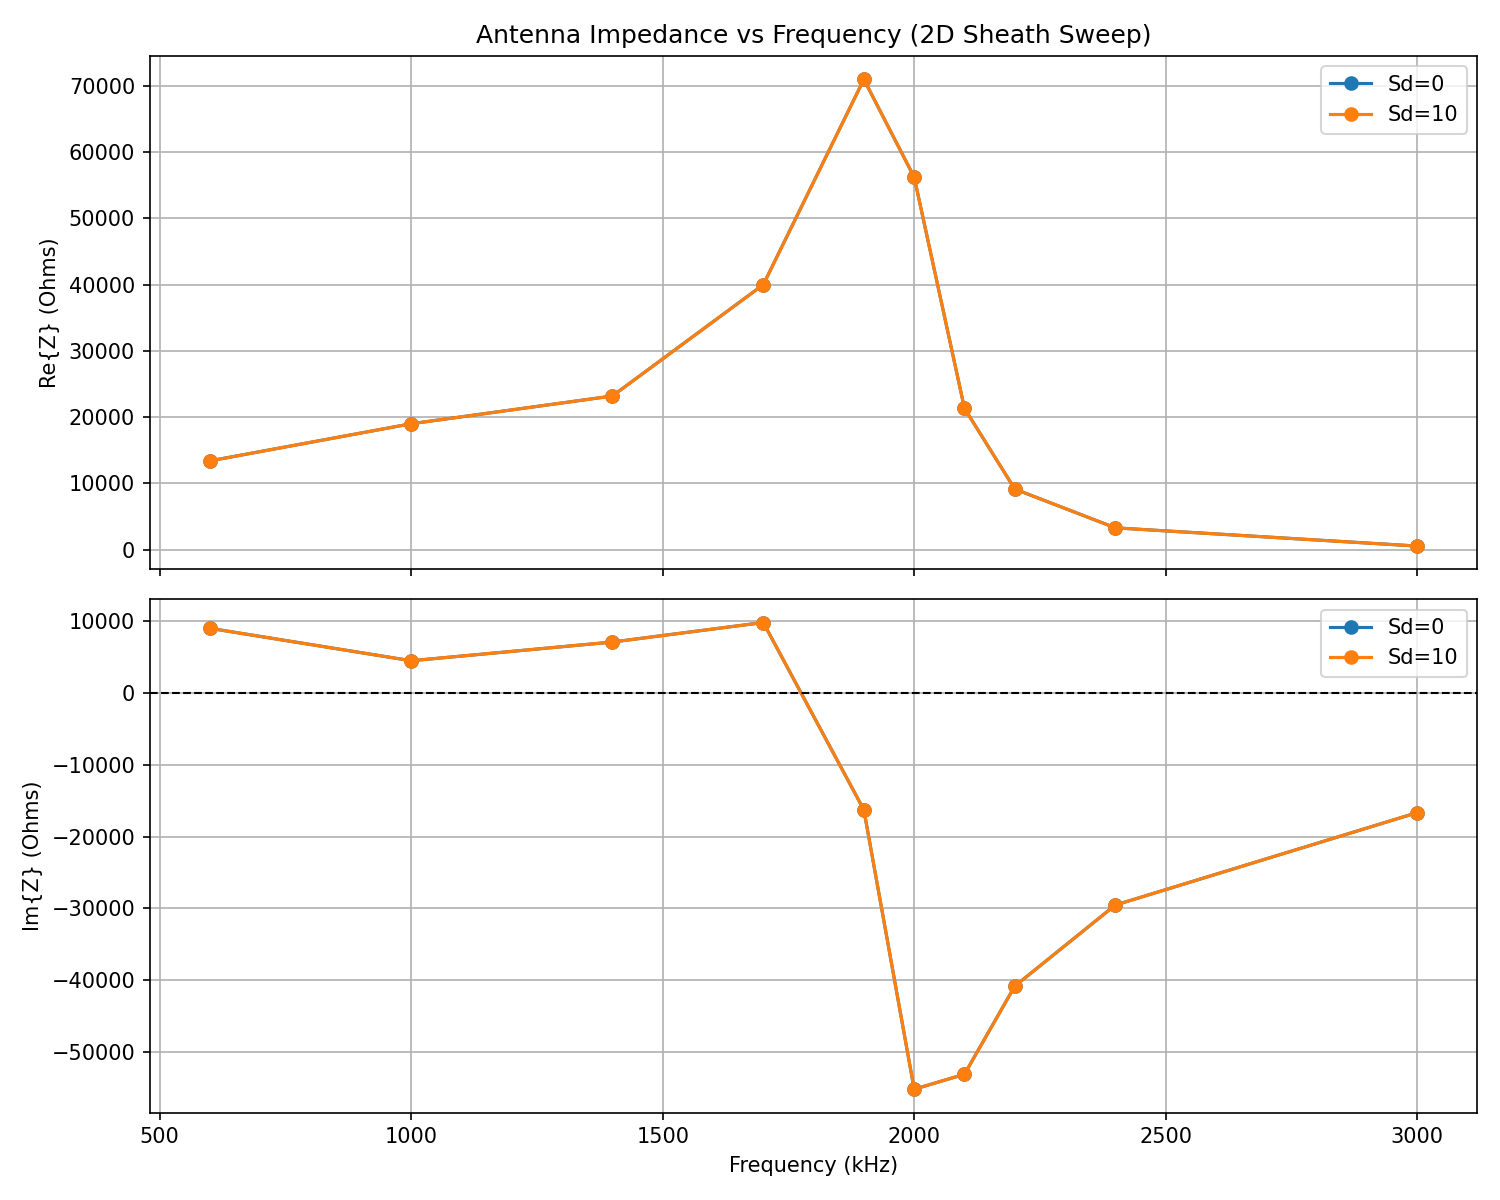
\includegraphics[width=0.9\textwidth]{sheath_2d_sweep_impedance.png}
\caption{CW \(\fp\)-screen impedance. \(\Sd=0\) and \(\Sd=10\) overlap at every point; \(\fres\approx\SI{1.775}{\mega\hertz}\) for both.}
\label{fig:fpscreen}
\end{figure}

\section{Interpretation}

The measurement problem of Chapter~\ref{ch:pulse} is solved. The remaining problem is in the model: a density hole exists somewhere, but not where \(V\) and \(I\) are formed. Chapter~\ref{ch:fix} dumps \(N_0\) along a line through the feed and finds that hole at the domain edge.

\chapter{Diagnosis and Coupling Fix}
\label{ch:fix}

\section{How the sheath was supposed to enter the model}

The active path is \texttt{src/physics/plasma.cpp}. Intended sequence:

\begin{enumerate}[leftmargin=1.5em]
\item Initialize \texttt{N0\_SPATIAL} to uniform bulk \(N_0\).
\item Set \(\mathrm{SIG}=1\) where plasma couples into Maxwell (\texttt{Ecalcmod}: \(-C_\mu\,\mathrm{SIG}\,J\)).
\item If \(\Sd>0\), dilate a distance field from a seed and set
\[
N_{0,\mathrm{spatial}}=N_0\cdot N_{\mathrm{MIN\_RATIO}}
\qquad (N_{\mathrm{MIN\_RATIO}}=10^{-6})
\]
for \(0<d\le\Sd\).
\item Fluid updates and current \(J\) use \texttt{N0\_SPATIAL}. Depleted cells give \(J\approx 0\).
\end{enumerate}

Feed observables (\texttt{src/source/source.cpp}) are a hard \(E_z\) voltage at \((35,35,33)\) and an Amp\`{e}re loop of \(B_x,B_y\) around that cell. Plasma loading of \(Z\) therefore requires depleted response in \emph{near-antenna} Yee nodes---not at the outer domain wall.

\section{Three overlapping mistakes}

\paragraph{Init order.}
\texttt{pffdtd.cpp} called \texttt{PLASMAclear()} \emph{before} \texttt{setup2()}. At that moment \texttt{ClearArrays()} had set \(\mathrm{ERX}=\mathrm{ERY}=\mathrm{ERZ}=1\) everywhere. The ``mark antenna / turn plasma on'' loop therefore set \(\mathrm{SIG}=1\) on the entire interior plasma box, not on the dipole.

\paragraph{Wrong sheath seed.}
Sheath dilation seeded from \(\mathrm{SIG}>0.5\). Even after reordering geometry, \(\mathrm{SIG}=1\) is defined where \emph{any} of \(\mathrm{ERX}/\mathrm{ERY}/\mathrm{ERZ}==1\). The thin-wire dipole in \texttt{sheath.str} is only \(\mathrm{ERZ}=0\) at \((35,35,20\text{--}45)\); \(\mathrm{ERX}\) and \(\mathrm{ERY}\) stay 1. So \(\mathrm{SIG}\) is a plasma-on mask, not a conductor mask. Distance \(d=0\) filled the whole interior; depletion landed in an \(\Sd\)-cell shell at the \emph{domain boundary} (\(\sim\SI{0.4}{\meter}\) for \(\Sd=10\), \(\Delta x=\SI{0.04}{\meter}\)), while the dipole sits at the grid center.

\paragraph{Overloaded \(\mathrm{SIG}\).}
\(\mathrm{SIG}\) was used as (a)~plasma--Maxwell coupling, (b)~sheath seed, and (c)~antenna density sink in \texttt{NBCcalc}. Those three meanings conflict. Near-antenna nodes kept bulk \(N_0\), so \(V\) and \(I\) were independent of \(\Sd\).

\section{Diagnostic: \(N_0\) along a line normal to the dipole}

A two-iteration dump of \texttt{N0\_SPATIAL} along \(i\) at \(j=35\), \(k=33\) (feed plane, \(+x\) normal to the \(z\)-dipole) is in \texttt{results/n0\_diag/}.

\paragraph{Before the fix} (legacy SIG-seeded binary). Both \(\Sd=0\) and \(\Sd=10\) show bulk \(N_0=4.96\times 10^{10}\,\mathrm{m}^{-3}\) next to the wire (\(i\approx 35\)). For \(\Sd=10\), depletion to \(N_0\times 10^{-6}\) appears only near the domain edge (\(i=1\ldots 5\)), outside the plasma box. A density hole exists, but the feed does not use those cells.

\begin{figure}[ht]
\centering
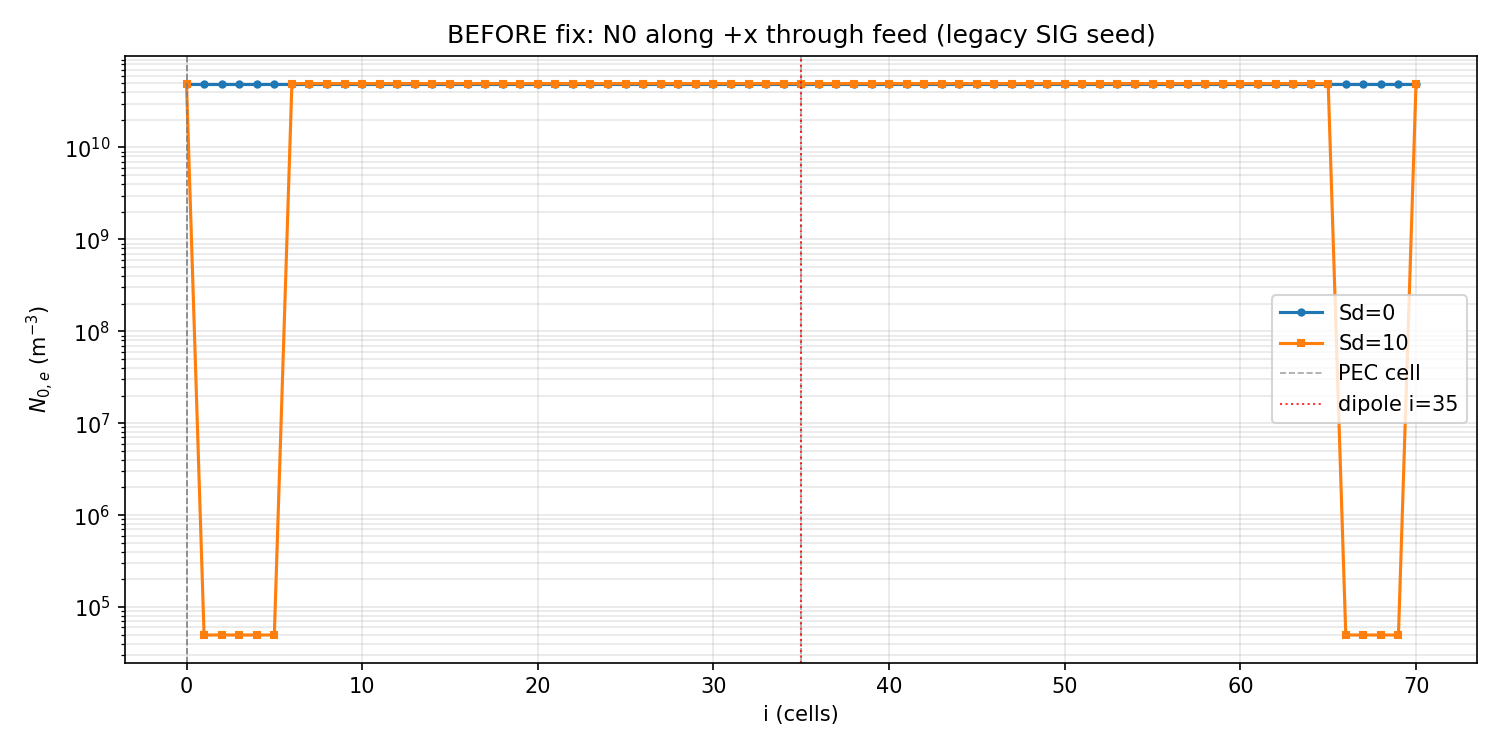
\includegraphics[width=0.9\textwidth]{n0_line_before.png}
\caption{\(N_0\) along a line through the feed, before the coupling fix. \(\Sd=10\) depletes the domain edge, not the wire.}
\label{fig:n0-before}
\end{figure}

\paragraph{After the fix.} Sheath seeds from 26 dipole PEC cells (not \(\sim\)14k false boundary PECs). \(\Sd=0\) is uniform bulk. \(\Sd=10\) depletes for \(0<|i-35|\le 10\); the domain edge remains bulk. Near-wire median \(N_0\): \(4.96\times 10^{10}\) (\(\Sd=0\)) versus \(4.96\times 10^{4}\) (\(\Sd=10\)).

\begin{figure}[ht]
\centering
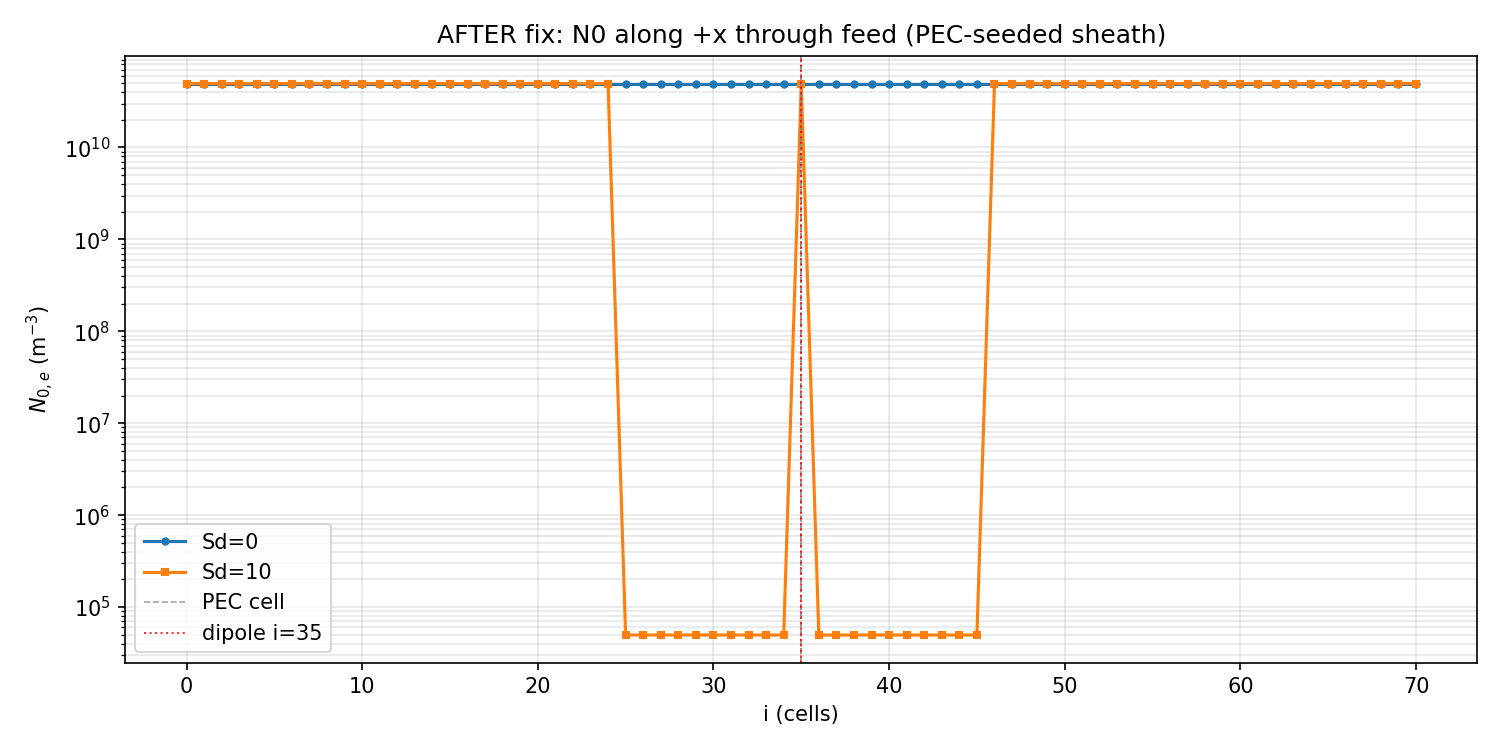
\includegraphics[width=0.9\textwidth]{n0_line_after.png}
\caption{\(N_0\) after the PEC-seeded fix. Depletion sits next to the wire for \(\Sd=10\).}
\label{fig:n0-after}
\end{figure}

\section{What changed in the code}

\begin{enumerate}[leftmargin=1.5em]
\item Reorder init in \texttt{pffdtd.cpp}: \texttt{ClearArrays} \(\to\) \texttt{setup2} (antenna \(\mathrm{ER*}\)) \(\to\) \texttt{PLASMAclear} \(\to\) \texttt{ApplySheath} \(\to\) \texttt{DumpN0Line} \(\to\) \texttt{Ninital}.
\item Seed the sheath from PEC cells (\(\mathrm{ERX}==0\) or \(\mathrm{ERY}==0\) or \(\mathrm{ERZ}==0\)), not from \(\mathrm{SIG}\).
\item Keep \(\mathrm{SIG}=1\) as plasma--Maxwell coupling only, including sheath cells. With depleted \(N_0\), \(J\approx 0\), so those cells act as vacuum.
\item Restrict the \texttt{NBCcalc} density sink to PEC cells.
\item Initialize the full \(0\ldots s_x\) index range in \texttt{ClearArrays} so uncleared \(i/j/k=0\) faces do not look like PEC (\(\sim\)14k bogus seeds \(\to\) 26 real dipole cells).
\item CLI \texttt{MaxIter} is re-applied after \texttt{setup1} reads the \texttt{.str} fail-safe line (previously ignored).
\item Path buffers enlarged so long \texttt{results/...} paths do not overflow.
\end{enumerate}

Legacy SIG-seeded dumps can be reproduced with \texttt{-DSHEATH\_LEGACY\_SIG\_SEED=1}. The next chapter confirms that feed impedance now depends on \(\Sd\).

\chapter{Post-Fix Confirmation}
\label{ch:confirm}

\section{CW confirm at the resonance shoulder}

A short CW check at \(\SI{1.7}{\mega\hertz}\) and \(\SI{1.9}{\mega\hertz}\), \(\Sd=0\) versus \(\Sd=10\), \(\fp=\SI{2}{\mega\hertz}\), \(\mathrm{MaxIter}=100000\), is in \texttt{results/sheath\_confirm\_z/}.

\begin{table}[ht]
\centering
\caption{Post-fix CW confirm. Relative change \(\lvert\Delta Z\rvert/\lvert Z_0\rvert\) was \(\sim 0.003\%\) before the fix.}
\label{tab:confirm}
\begin{tabular}{@{}rrrrrr@{}}
\toprule
\(f\) (MHz) & \(\ReZ\) \(\Sd{=}0\) & \(\ReZ\) \(\Sd{=}10\) & \(\ImZ\) \(\Sd{=}0\) & \(\ImZ\) \(\Sd{=}10\) & \(\lvert\Delta Z\rvert/\lvert Z_0\rvert\) \\
\midrule
1.70 & 39564 & 6406 & $+10023$ & $-21936$ & 112.8\% \\
1.90 & 71059 & 4573 & $-15542$ & $-22129$ & 91.9\% \\
\bottomrule
\end{tabular}
\end{table}

\begin{figure}[ht]
\centering
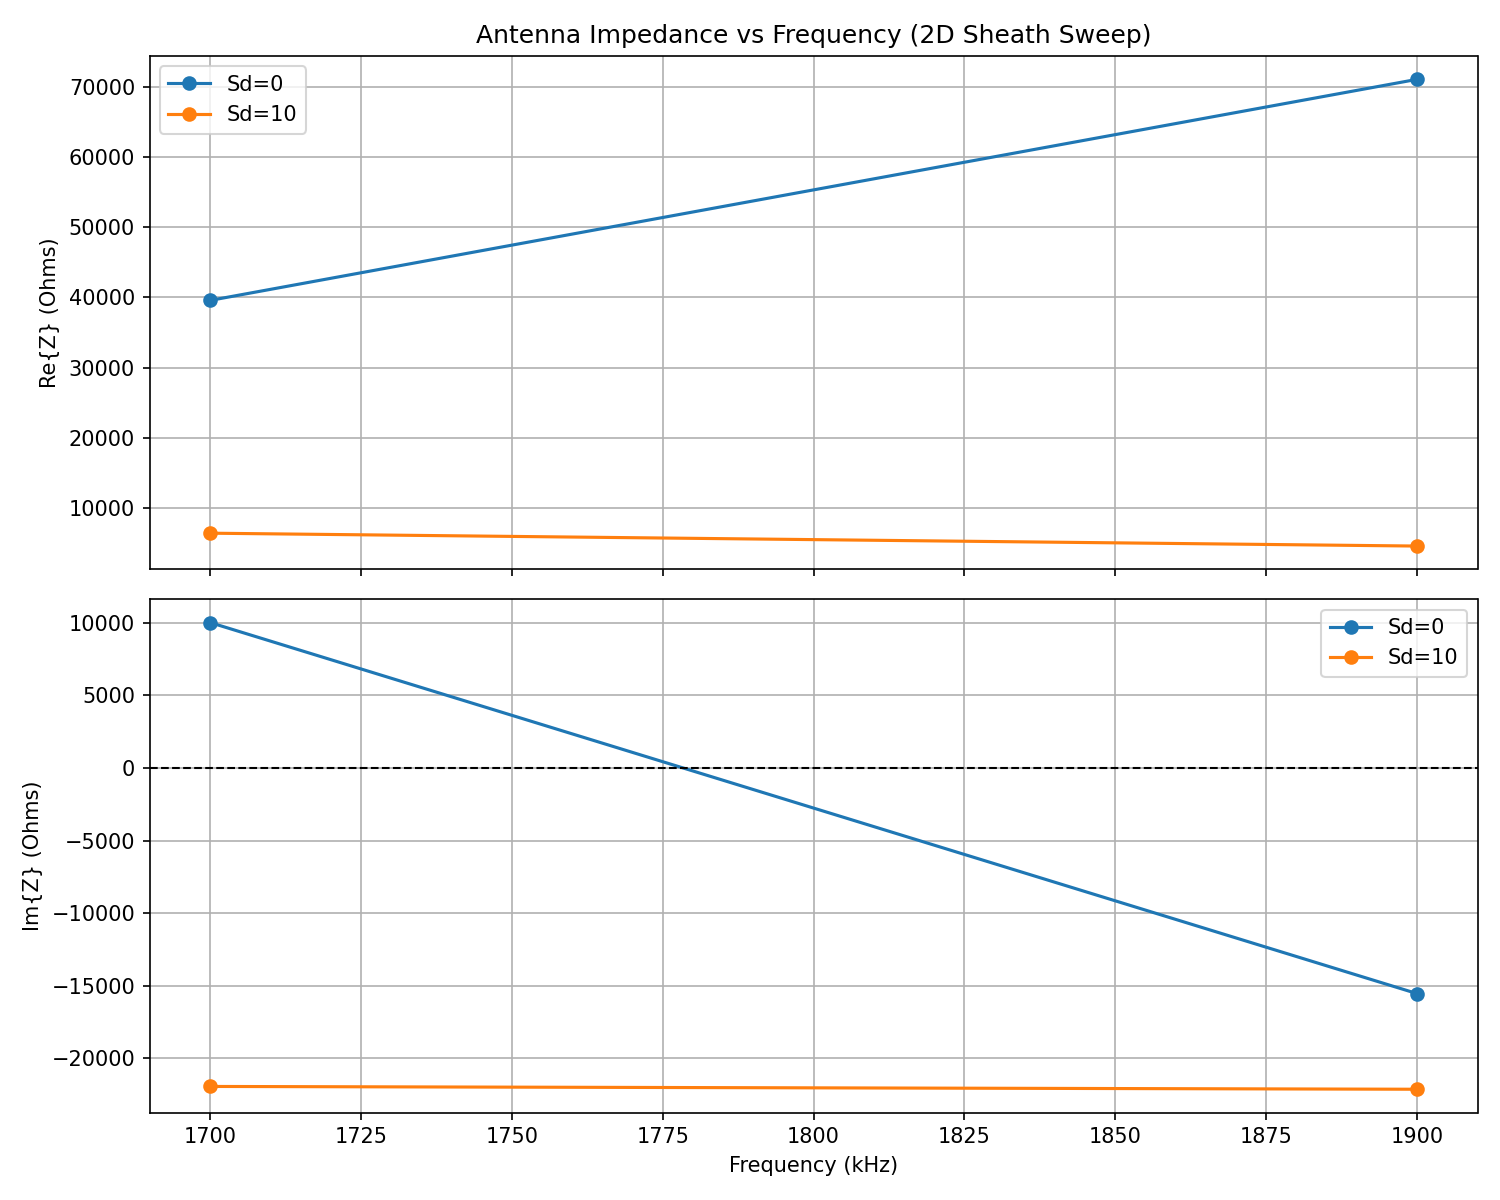
\includegraphics[width=0.9\textwidth]{confirm_z_impedance.png}
\caption{Post-fix CW impedance at 1.7 and 1.9~MHz. \(\Sd=0\) still crosses \(\ImZ=0\) between the two points; \(\Sd=10\) is capacitive at both.}
\label{fig:confirm}
\end{figure}

\paragraph{Succeeded.} Impedance now depends strongly on sheath width. \(\Sd=0\) still shows an \(\ImZ\) sign change between 1.7 and 1.9~MHz (\(\fres\sim\SI{1.78}{\mega\hertz}\)). \(\Sd=10\) is strongly capacitive at both frequencies: the feed sees the vacuum sheath. The coupling bug is resolved.

\paragraph{Still open.} Two frequencies cannot locate the new \(\fres\) for every \(\Sd\). A dense CW grid is required for a Tu shift curve (Chapter~\ref{ch:cwtu}).

\section{Post-fix long pulse FFT}

A full \(\Sd\) grid after the fix is in \texttt{results/sheath\_pulse\_long/} (\(\fp=\SI{2}{\mega\hertz}\), Spar \(\SI{2}{\mega\hertz}\), \(\mathrm{MaxIter}=2\times 10^{5}\), \(\mathrm{VcRate}=50\)). Wall time 6.57~h; all six cases exited 0. Analyzer: \texttt{scripts/analyze\_pulse\_long.py}, using CW-compatible \(+\) to \(-\) crossings in 1.2--3~MHz.

\begin{table}[ht]
\centering
\caption{Post-fix pulse FFT. Automatic picks are noisy; \(\mathrm{d}f\sim\SI{75}{\kilo\hertz}\).}
\label{tab:pulse-long}
\begin{tabular}{@{}rrrr@{}}
\toprule
\(\Sd\) & \(\fres\) (MHz), Im \(+\!\to\!-\) in 1.2--3~MHz & \(\ImZ\) at 1.7~MHz & \(\ImZ\) at 1.9~MHz \\
\midrule
0  & 2.09 & $+18325$ & $+22444$ \\
2  & 1.23 (noisy; also 2.03) & $-536$ & $+1115$ \\
4  & 2.02 & $-1542$ & $+8541$ \\
6  & 2.02 & $-4527$ & $+8638$ \\
8  & 2.00 & $-7910$ & $+3205$ \\
10 & 2.00 & $-15393$ & $-29243$ \\
\bottomrule
\end{tabular}
\end{table}

\begin{figure}[ht]
\centering
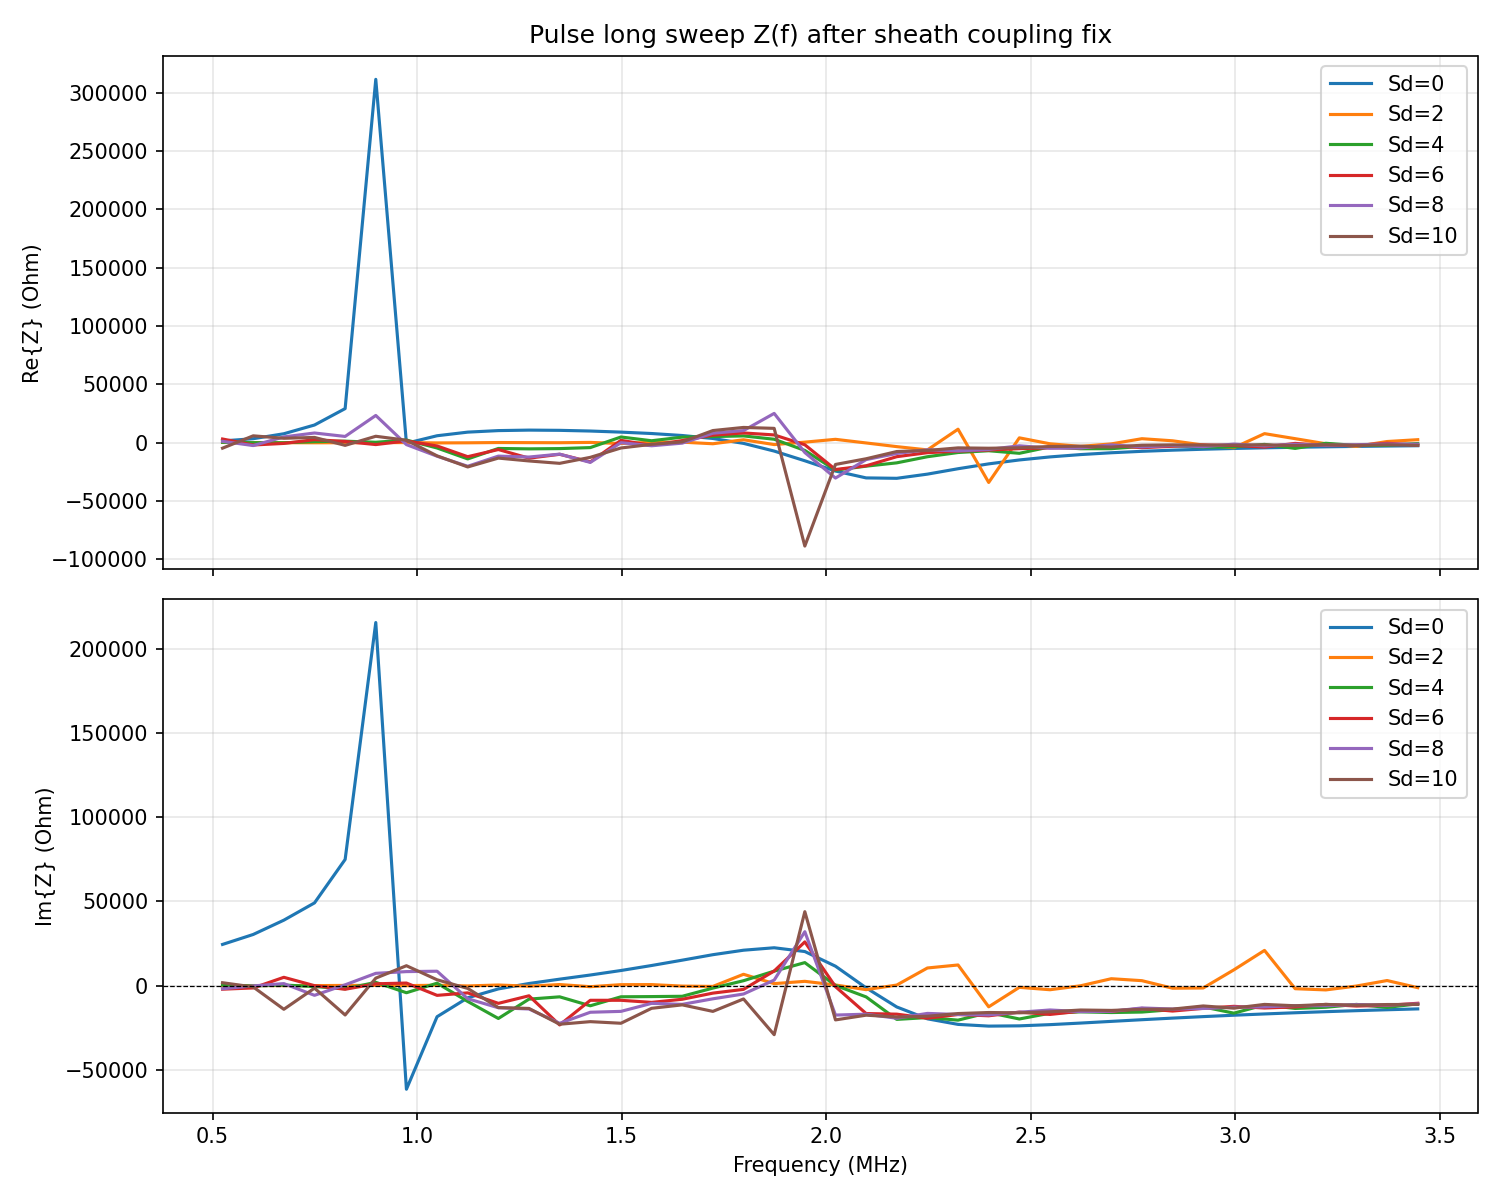
\includegraphics[width=0.9\textwidth]{pulse_long_impedance.png}
\caption{Post-fix pulse FFT impedance. Curves separate with \(\Sd\); \(\Sd=10\) is capacitive through 1.7--1.9~MHz, matching the CW confirm.}
\label{fig:pulse-long-z}
\end{figure}

\begin{figure}[ht]
\centering
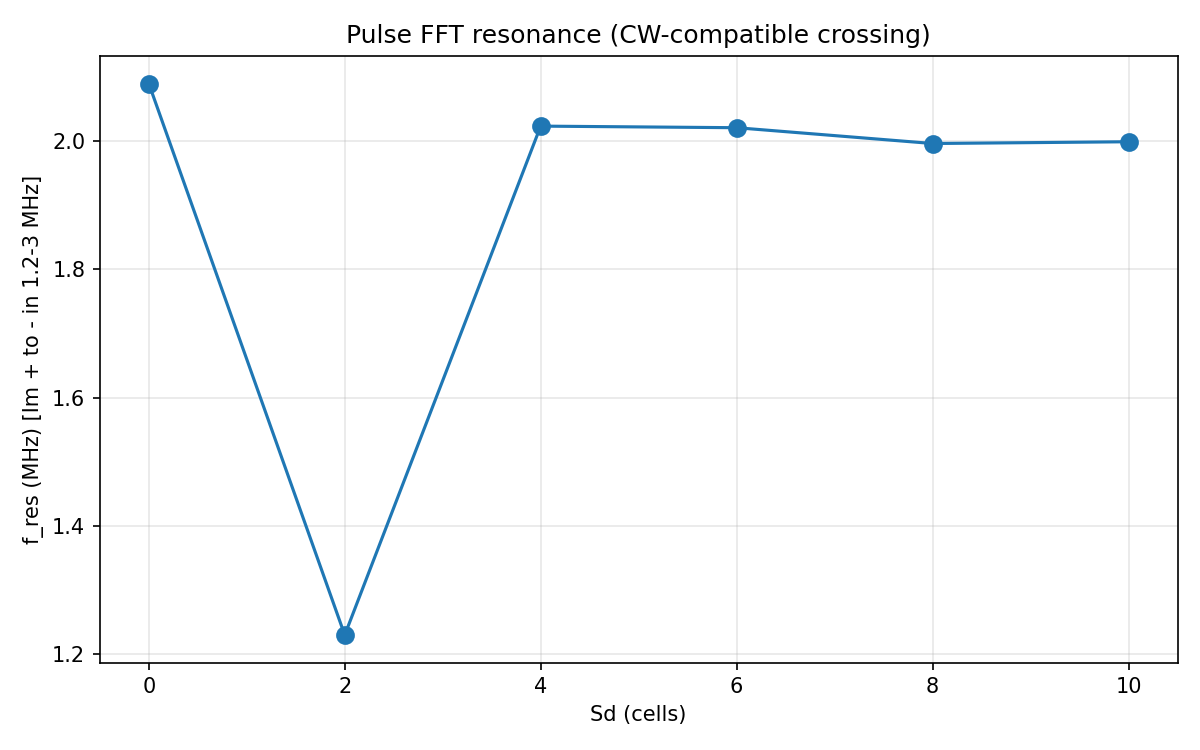
\includegraphics[width=0.85\textwidth]{pulse_long_resonance_shift.png}
\caption{Pulse-FFT resonance versus \(\Sd\). Frequency resolution is too coarse for a Tu curve; CW remains the preferred \(\fres\) measurement.}
\label{fig:pulse-long-shift}
\end{figure}

\paragraph{Succeeded.} Pulse FFT now \emph{sees} \(\Sd\). \(\Sd=10\) capacitive at 1.7--1.9~MHz matches the CW confirm.

\paragraph{Failed as a precision tool.} Stock \(-\) to \(+\) resonance picks are often spurious. Even with \(+\) to \(-\) crossings, \(\mathrm{d}f\sim\SI{75}{\kilo\hertz}\) is too coarse to map a clean \(\fres(\Sd)\) curve. A denser CW sweep is the remaining measurement.

\chapter{Dense CW Tu Sweep}
\label{ch:cwtu}

\section{Campaign setup}

The dense CW grid was the post-fix measurement intended to produce a clean \(\fres(\Sd)\) curve. Driver: \texttt{scripts/run\_sheath\_cw\_tu.ps1}. Output: \texttt{results/sheath\_cw\_tu/} (voltage/current only; no field dumps).

\begin{itemize}[leftmargin=1.5em]
\item \(\Sd\in\{0,2,4,6,8,10\}\).
\item Drive frequencies: 1.50, 1.60, 1.70, 1.75, 1.80, 1.85, 1.90, 2.00, 2.10, 2.20, 2.30~MHz (66 cases).
\item \(\fp=\SI{2}{\mega\hertz}\), template \texttt{sheath\_sine\_vc.str}, \(\mathrm{MaxParallel}=3\), \(\mathrm{OMP}=4\).
\item Started 13 August 2026 12:48; all 66 cases finished by 18 August 2026.
\end{itemize}

Analyzer: \texttt{scripts/analyze\_cw\_tu\_partial.py} (last-50\% phasor \(Z\), same convention as the \(\fp\)-screen; series resonance is the first \(\ImZ\) \(+\) to \(-\) crossing). Tables and figures: \texttt{paper0_sheath_campaign/analysis/data/cw\_tu\_*.txt}, \texttt{paper0_sheath_campaign/analysis/figures/cw\_tu\_*.png}.

\section{Campaign status}

As of 18 August 2026: \textbf{66 complete, 0 running, 0 pending}, 0 failed. Every planned cell in Table~\ref{tab:cwtu-status} finished with a full \texttt{data.vc} file.

The \(\Sd=0\), 1.50~MHz case was skipped once by the orchestrator on restart; its file is smaller than the others and lacks a \texttt{DONE} line, but the phasor at 1.50~MHz is consistent with the rising inductive branch below the crossing and is included in the plots.

\begin{table}[ht]
\centering
\caption{CW Tu case status (18 August 2026). All cells complete.}
\label{tab:cwtu-status}
\scriptsize
\begin{tabular}{@{}rccccccccccc@{}}
\toprule
\(\Sd\) & 1.50 & 1.60 & 1.70 & 1.75 & 1.80 & 1.85 & 1.90 & 2.00 & 2.10 & 2.20 & 2.30 \\
\midrule
0  & C & C & C & C & C & C & C & C & C & C & C \\
2  & C & C & C & C & C & C & C & C & C & C & C \\
4  & C & C & C & C & C & C & C & C & C & C & C \\
6  & C & C & C & C & C & C & C & C & C & C & C \\
8  & C & C & C & C & C & C & C & C & C & C & C \\
10 & C & C & C & C & C & C & C & C & C & C & C \\
\bottomrule
\end{tabular}
\end{table}

\section{Impedance versus frequency}

Figure~\ref{fig:cwtu-z} and Table~\ref{tab:cwtu-z} show the full-grid phasor results. Unlike the pre-fix \(\fp\)-screen, curves for different \(\Sd\) are well separated across 1.50--2.30~MHz.

\begin{figure}[ht]
\centering
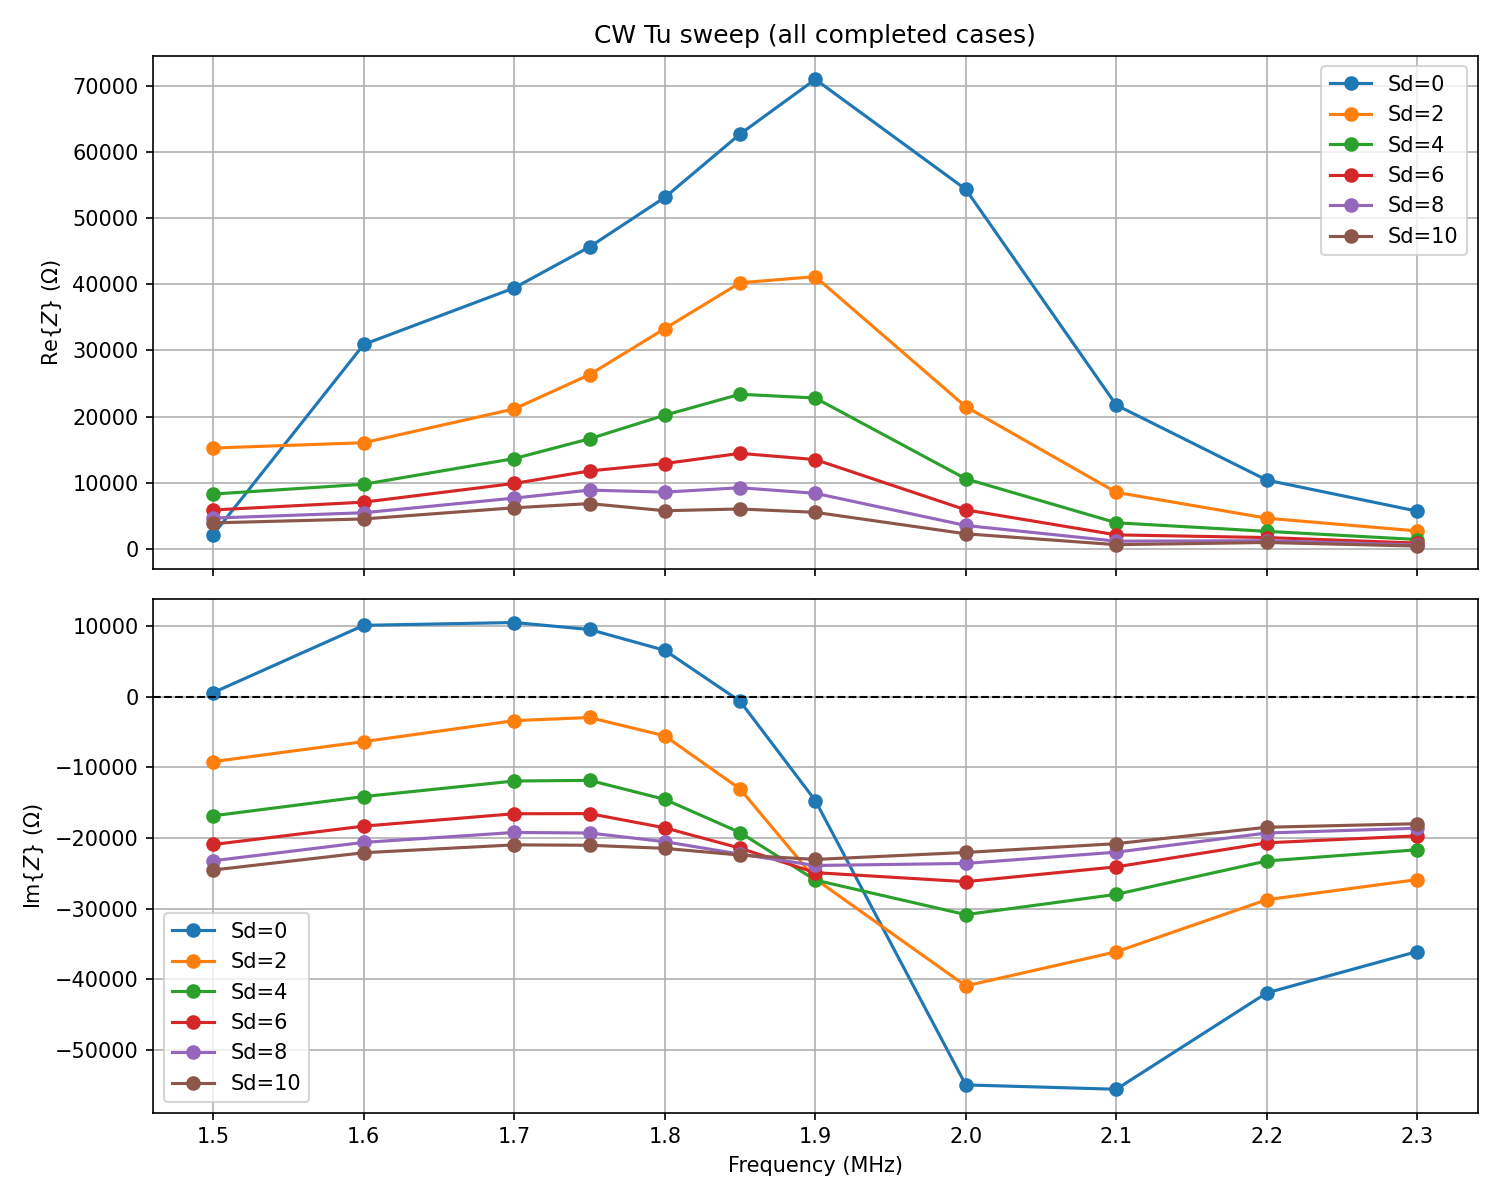
\includegraphics[width=0.92\textwidth]{cw_tu_impedance.png}
\caption{CW Tu sweep, all 66 cases. \(\Sd=0\) crosses \(\ImZ=0\) near 1.85~MHz and is capacitive above \(\sim\SI{2.0}{\mega\hertz}\). Every \(\Sd\ge 2\) curve stays capacitive (\(\ImZ<0\)) across the entire band.}
\label{fig:cwtu-z}
\end{figure}

\begin{table}[ht]
\centering
\caption{Selected phasor impedances (\(\si{\ohm}\)). Full table: \texttt{paper0_sheath_campaign/analysis/data/cw\_tu\_summary.txt}.}
\label{tab:cwtu-z}
\begin{tabular}{@{}rrrrr@{}}
\toprule
\(f\) (MHz) & \(\Sd\) & \(\ReZ\) & \(\ImZ\) & note \\
\midrule
1.50 & 0  & 2130  & $+585$   & inductive shoulder \\
1.85 & 0  & 62775 & $-640$   & just past crossing \\
2.00 & 0  & 54406 & $-54920$ & capacitive above \(\fres\) \\
1.50 & 2  & 15227 & $-9181$  & capacitive at band edge \\
2.00 & 2  & 21484 & $-40907$ & still capacitive \\
1.70 & 10 & 6182  & $-20959$ & matches confirm-Z \\
2.00 & 10 & 2238  & $-22032$ & \(\lvert Z\rvert\) lowest in band \\
\bottomrule
\end{tabular}
\end{table}

\section{\texorpdfstring{Series resonance $\fres(\Sd)$}{Series resonance f\_res(Sd)}}

Linear interpolation of the \(\Sd=0\) \(+\) to \(-\) crossing between 1.80 and 1.85~MHz gives
\begin{equation}
\fres(\Sd=0)\approx\SI{1.846}{\mega\hertz}.
\label{eq:cwtu-fres0}
\end{equation}
That matches the post-fix confirm (sign change between 1.7 and 1.9~MHz) and is slightly above the coarse pre-fix 1.7/1.9 interpolation (\(\sim\SI{1.775}{\mega\hertz}\)).

For \(\Sd=2,4,6,8,10\), \(\ImZ<0\) at \emph{every} frequency in 1.50--2.30~MHz. No \(+\) to \(-\) crossing appears anywhere in the grid for \(\Sd>0\). Any series crossing for those cases therefore lies \emph{below} \(\SI{1.50}{\mega\hertz}\)---the opposite direction from Tu~\cite{tu2008}, which predicts \(\fres\) moving \emph{upward} with \(\Sd\) toward the free-space value. Figure~\ref{fig:cwtu-res} contains only the \(\Sd=0\) point.

\begin{figure}[ht]
\centering
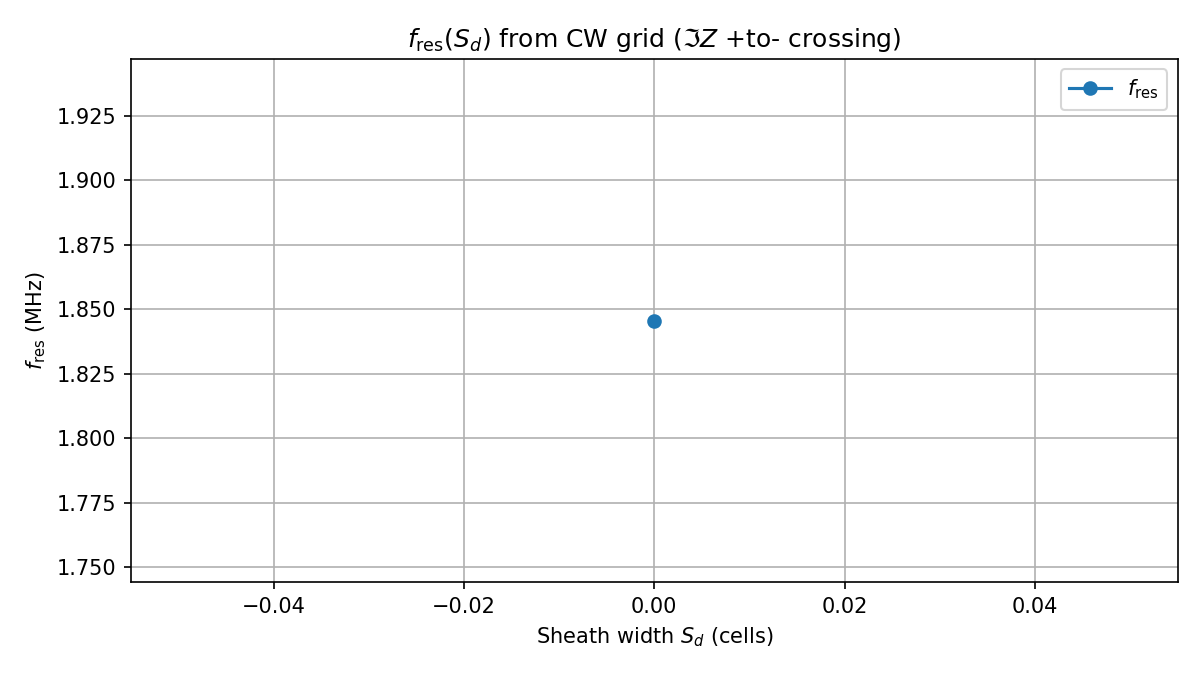
\includegraphics[width=0.85\textwidth]{cw_tu_resonance.png}
\caption{\(\fres(\Sd)\) from the full CW grid (\(\ImZ\) \(+\) to \(-\) crossing). Only \(\Sd=0\) has a crossing in 1.50--2.30~MHz.}
\label{fig:cwtu-res}
\end{figure}

Table~\ref{tab:cwtu-res} summarizes the resonance extraction. The high-frequency extension (1.90--2.30~MHz) rules out the provisional hypothesis from the partial run that a Tu-like upward crossing might appear above 1.9~MHz for large \(\Sd\): \(\Sd=10\) remains strongly capacitive at 2.0 and 2.3~MHz.

\begin{table}[ht]
\centering
\caption{Series resonance from \(\ImZ\) \(+\) to \(-\) crossings.}
\label{tab:cwtu-res}
\begin{tabular}{@{}rll@{}}
\toprule
\(\Sd\) & \(\fres\) & note \\
\midrule
0  & \(\SI{1.846}{\mega\hertz}\) & crossing in 1.50--2.30~MHz band \\
2  & --- & all \(\ImZ<0\); crossing at or below 1.50~MHz \\
4  & --- & all \(\ImZ<0\); crossing at or below 1.50~MHz \\
6  & --- & all \(\ImZ<0\); crossing at or below 1.50~MHz \\
8  & --- & all \(\ImZ<0\); crossing at or below 1.50~MHz \\
10 & --- & all \(\ImZ<0\); crossing at or below 1.50~MHz \\
\bottomrule
\end{tabular}
\end{table}

\section{What succeeded}

\begin{itemize}[leftmargin=1.5em]
\item Coupling is visible in CW at every \(\Sd>0\): \(Z(f)\) is no longer independent of sheath width.
\item The \(\Sd=0\) plasma-loaded resonance is resolved to \(\sim\SI{50}{\kilo\hertz}\) spacing near \(\fp\).
\item The full grid confirms the post-fix confirm-Z picture: \(\Sd=0\) is inductive below \(\sim\SI{1.85}{\mega\hertz}\); \(\Sd=10\) is capacitive everywhere in the band.
\end{itemize}

\section{What did not match the upward-shift target}

The campaign design target---inspired by a circuit reading of Tu~\cite{tu2008}---was an \emph{upward} shift of \(\fres\) with \(\Sd\). That shift was not reproduced in this band:

\begin{itemize}[leftmargin=1.5em]
\item Only \(\Sd=0\) yields a measurable in-band series crossing.
\item Wider sheaths add capacitive loading (\(\lvert Z\rvert\) falls with \(\Sd\) at fixed \(f\)) but do not move a \(+\) to \(-\) crossing upward through 1.50--2.30~MHz.
\item If the same crossing definition applies to \(\Sd\ge 2\), the feature has moved \emph{downward} relative to \(\Sd=0\), or the feed impedance is dominated by series sheath capacitance without a clear in-band LC crossing.
\end{itemize}

Follow-up completed in Chapter~\ref{ch:lowf}: the CW grid was extended below 1.50~MHz for \(\Sd=0,2,10\). That campaign locates \(\fres(\Sd=2)\approx\SI{0.655}{\mega\hertz}\) and finds \(\Sd=10\) capacitive down to \(\SI{0.50}{\mega\hertz}\), confirming the downward trend. Interpretation (series \(C_{\mathrm{sh}}\) vs dielectric unloading; Balmain--Liu lineage; Tu regime mismatch): \texttt{paper0_sheath_campaign/analysis/tu\_discrepancy\_discussion.md} and Chapter~\ref{ch:status}.

\chapter{Status and Next Steps}
\label{ch:status}

\section{Where the campaign stands}

The work from February through 18 August 2026 is one antenna-in-plasma story on a single dipole grid.

\begin{enumerate}[leftmargin=1.5em]
\item \textbf{February baseline.} Free-space versus plasma impedance is measurable. Same geometry as all later sheath runs.
\item \textbf{May pulse \(\Sd\) sweep.} Failed as a measurement (no usable \(\fres\); GHz FFT artifacts). Independently, the sheath was not on the wire.
\item \textbf{Low-frequency CW.} Measurement method works; frequencies sit below resonance; \(Z\) still independent of \(\Sd\).
\item \textbf{CW \(\fp\)-screen.} Measurement success (\(\fres\approx\SI{1.775}{\mega\hertz}\)) and physics failure (\(Z(\Sd=0)\equiv Z(\Sd=10)\) to \(\sim 0.003\%\)). Negative control, keep the folder.
\item \textbf{Coupling fix.} Sheath had been seeded from the plasma-on mask before PEC existed; depletion sat at the domain edge. PEC-seeded \texttt{ApplySheath} after \texttt{setup2} puts the hole next to the wire.
\item \textbf{Post-fix confirm.} \(\lvert\Delta Z\rvert/\lvert Z\rvert\sim 90\)--\(110\%\) at 1.7/1.9~MHz. Pulse FFT now sees \(\Sd\) but is too coarse for a Tu curve.
\item \textbf{Dense CW (complete).} All 66 cases finished. \(\fres(\Sd=0)\approx\SI{1.846}{\mega\hertz}\). \(\Sd\ge 2\) is capacitive at every point in 1.50--2.30~MHz. The Tu upward shift of \(\fres\) with \(\Sd\) was not reproduced with the \(+\) to \(-\) \(\ImZ\) crossing definition.
\end{enumerate}

\section{Open items}

\begin{enumerate}[leftmargin=1.5em]
\item Extend the CW grid \emph{below} 1.50~MHz for \(\Sd\ge 2\) to locate any \(+\) to \(-\) crossings outside the August band, or adopt an alternative resonance marker when the feed is uniformly capacitive.
\item Compare \(\fres(\Sd=0)\) and any low-frequency crossings to the free-space resonance on the same dipole grid.
\item Optional: longer muted pulse (\(\mathrm{MaxIter}\gtrsim 10^{6}\)) if additional frequency resolution is needed outside CW.
\item Optional: re-run the \(\fp\)-screen with the fixed physics as a published before/after pair. Confirm-Z and the CW Tu grid already show coupling; this is documentation, not debugging.
\item Software not in this report's critical path: GPU, MPI, broader unit-test coverage.
\end{enumerate}

\section{Data map}

\begin{table}[ht]
\centering
\caption{Primary data and writeups for each phase.}
\label{tab:datamap}
\begin{tabular}{@{}lll@{}}
\toprule
Phase & Results & Notes / figures \\
\midrule
Feb baseline & \texttt{results/freespace\_test}, \texttt{ionoplasma\_*} & Ch.~\ref{ch:february} \\
Pulse \(\Sd\) & \texttt{results/sheath\_sweep}, \texttt{sheath\_long} & \texttt{analysis/sheath\_coupling\_findings.md} \\
Narrow / 2D CW & \texttt{results/sheath\_narrow\_band}, \texttt{sheath\_2d\_sweep} & Ch.~\ref{ch:narrow} \\
\(\fp\)-screen & \texttt{results/sheath\_fp\_screen} & pre-fix negative control \\
\(N_0\) dump & \texttt{results/n0\_diag} & \texttt{analysis/figures/n0\_line\_*.png} \\
Confirm & \texttt{results/sheath\_confirm\_z}, \texttt{sheath\_pulse\_long} & Ch.~\ref{ch:confirm} \\
CW Tu & \texttt{results/sheath\_cw\_tu} & Ch.~\ref{ch:cwtu}; \texttt{analysis/data/cw\_tu\_*.txt} \\
\bottomrule
\end{tabular}
\end{table}

The coupling-fix narrative in \texttt{analysis/sheath\_coupling\_findings.md} remains the detailed laboratory note; this report is the chronological account intended for sharing as PDF.


\begin{thebibliography}{9}
\bibitem{tu2008}
W.~Tu, J.-L.~Pathak, and R.~F.~Benson,
\textit{Plasma sheath structures around a radio frequency antenna},
J.\ Geophys.\ Res., 2008.
A local copy is in \texttt{../../docs/references/Tu2008\_JGR\_plasma\_sheath.pdf}.

\bibitem{ward2006}
J.~D.~Ward,
\textit{Plasma Frequency Probe Design and Implementation},
Master's thesis, Utah State University, 2006.
\end{thebibliography}

\end{document}
